% Title and author information 
\title{ON THE INTERFEROMETRY OF LAZER BEAMS}
\author{
    Eduardo Barroso \address{1} \\[0.3em]
    {\scriptsize
        \address{1} Department of Physics Engineering; Monterrey Institute of Technology, Monterrey, N.L 64849.\\
    }
}
\date{\today}


\setabstract{
    The development of vector calculus in the midst of the XIX century gave rise to very complete models for describing waves. 
    For classical physics, applying these models to the phenomenon known as light became the bedrock of what is now the field of optics. One property of these models is that they allow for two light beams to interact leading to a whole discussion involving phases, frequencies, amplification and total annihilation. 
    In this work, the principal elements used to build a amplitude division interferometer are presented and explained. Furthermore, a brief discussion on the principles of interferometfy is included to serve as a stepping stone towards exposing our results in the last section.  
}

\maketitle


\section{Introduction}
\label{sec:INTRO}
Quantum electrodynamics provides the most fundamental description of light up to date. However, the classical formulation developed in the early years of this field yields a very elegant, intuitive and simple understanding of light. Furthermore, the mathematical models built around this classical theory are tailor made for the level of the physical experimentation discussed in this work. From this classical standpoint, light can be considered to be a harmonic solution (wave) to the second order, linear and partial differential equation derived from Maxwell's equations \cite{maxwell1954electricity}. Because of this considerations, we expect for light to exhibit wave like properties. \\

One of such properties is interference. By interfering two light beams, it is possible for the emerging beam to sum up constructively, destructively or some state in the middle (Figure \ref{fig:BasicInterf}). The parameter that primarily governs interference is the phase of the wave. However, it is important to keep track of the amplitudes when constructing optical experiments because in order for interference to occur a series of conditions must hold.  In the case of the electromagnetic waves, the conditions for interference are that the light source must be monochromatic, coherent and polarized in the same orientation. \\

This work aims to explain the basic experimental considerations that need surveillance when working with interferometers. This is done by designing and implementing a type of amplitude splitting interferometer known as Mach-Zhender. Later, a series of measurements and modifications are implemented to characterize the phenomena known as interference.





\section{Materials}
\label{sec:mat}
\begin{enumerate}
    \item LASER HeNe (633nm, 15mW)
    \item 2 Linear Polarizators.
    \item 2 Beam splitters of cubic type.
    \item 1 Retarder of half wavelength.
    \item Camara. 
    \item Fixed Optic Mounts.
    \item 4 Mirrors.
    \item 1 Collimator.
    \item 1 Pupil.
    \item Security Glasses.
\end{enumerate}

\section{Theoretical Framework}
\label{sec:TEO_FRAMEWORK}
%%%%%%%%%%%%%%%%%%%%%%%%%%%%%
In the early XIX century when Augustin-Jean Fresnel performed Thomas Young experiment, he proved empirically that light behaves like a wave. The results disproved the generally accepted corpuscular theory of light developed by Newton. This lead to the devolpment of a wave theory of light that ended up with Maxwell's equations \cite{maxwell1954electricity}. This set of 4 equations, describes how electromagnetic waves behave under any circumstance. \\

Few mathematical treatment is required to derive a wave equation that all electromagnetic waves must obey. The result 
\begin{equation}
    \frac{\partial^2 u}{\partial z^2} = \frac{1}{v^2}\frac{\partial^2 u}{\partial t^2},
    \label{eq:wave_eqn}
\end{equation}
 gives rise to a family of solutions that satisfy the super-position principle \footnote{The sum of two solutions to equation \ref{eq:wave_eqn} is also a solution to the wave equation.}. This principle, is the cornerstone that enable mathematics to describe the interaction of two light beams predicted by Young 220 years ago.  

\subsection{INTERFERENCE}
Interference is the phenomena associated to the sum of waves and the interaction of light itself. Thus, the work proceeds to define interference as the vector sum of the amplitudes of two light waves. Figure \ref{fig:BasicInterf} illustrates the sum of 3 sets of waves. The first row is called constructive interference where the amplitudes magnify each other. The second row is a visualization of destructive interference \footnote{Encountering annihilation in our models is not good for physicists because keep in mind that light is a natural system ruled by conservation laws. Thus, this case brings to question: what happens with that conservation of energy in a case of two light waves? Turns out, energy is simply distributed in a different configuration.}  where a maximum of a wave interferes with a minimum of the other canceling each other out. The last row is a case that is nether total constructive nor destructive interference. \\

\begin{figure}[H]
    \centering
    \includegraphics[scale=0.30]{Figures/Figures_I/Basic_Interference.jpg}
    \caption{1) Constructive Interference of A and B, 2) Destructive interference of A and B, 3) Partial constructive interference of A and B. }
    \label{fig:BasicInterf}
\end{figure}

It is important to mention that a series of characteristics have to hold for a optical system to interfere. To further understand these considerations, consider the vector sum of two light waves:  $\Vec{E_1}=E_1 exp(i[\vec{k_1}\cdot \vec{r}-wt+\epsilon_1])$ and $\Vec{E_2}=E_2 exp(i[(\vec{k_2}\cdot \vec{r}-wt+\epsilon_2])$. The resulting sum, averaged over time \footnote{This measurable quantity is calculated by taking a mean value over time of the energy of the field. This leads to the relation $I = \langle E \cdot E \rangle$} is
\begin{equation}
    I_{tot} = I_1 + I2 + 2 cos(\delta),
    \label{eq:interf}
\end{equation}
where $\delta = (\vec{k_2}-\vec{k_1})\cdot \vec{r} + (\epsilon_1-\epsilon_2)$. Result \ref{eq:interf} hints at the fact that $w, k, E_i$ and polarization play a critical role in that collectively create the phenomena of interference. The characteristics are summarized as follows. For electromagnetic waves to interact they must: 
\begin{itemize}
    \item be monochromatic.
    \item be coherent (temporal coherence). 
    \item share a polarization state.
\end{itemize}

Figure \ref{fig:VectorInterf} is an excellent visualization of this result.However in a macroscopic characterization, the important takeaway is that the directional difference between  $\vec{k_1} $ and $\vec{k_2}$ controls the number of fringes in displayed in figure \ref{fig:Interf_Types}. 

\begin{figure}[H]
    \centering
    \includegraphics[scale=0.30]{Figures/Figures_I/Vectorsum_Interference.png}
    \caption{Vector Sum of two electromagnetic waves \cite{hecht1987optics}}
    \label{fig:VectorInterf}
\end{figure}

%%%%%%%%%%%%%%%%%%%%%%%%%%%%%
\subsection{TEMPORAL COHERENCE}
The measurement of coherence is a comparison between the relative phases of two light waves \cite{guenther2015modern}. As of 2021 every realistic source of light has an associated bandwidth of temporal frequencies. This means that for the case of our LASER is not perfectly monochromatic. The implications of this fact permits us to invoke Heisenberg uncertainty principle 
\begin{equation} 
\Delta E \Delta t\ge \hbar/2 ,
\end{equation} 
Where $\hbar$ is Planks constant. The size of this bandwidth is related to $\Delta E$ and temporal coherence($\tau$) is related to $\Delta t$. The key takeaway is that for more monochromatic beams more temporal coherence they are allowed to have. 

The mathematical analysis of such statement can be done with Fourier transforms. It all borrows down to introducing the mutual coherence function ($\gamma$)
\begin{equation}
 \gamma (\tau) = \frac{\Gamma(\tau)}{\Gamma(0)},
\end{equation}
where 
\begin{equation}
 \Gamma (\tau) = \int_0^{\infty} E_0(\tau)^2 exp(-iw\tau) dw,
\end{equation}
relates bandwidth with coherence ($\tau$). Also note the last results is a Fourier transform. 

%%%%%%%%%%%%%%%%%%%%%%%%%%%%%
\subsection{INTERFEROMETERS}
In the most general sense, any interferometer works by either dividing its wavefront or its amplitude. In the case of wavefront division, a point-like source emits a wave and a physical barrier is applied to filter only some selected parts of the wavefront (Figure \ref{fig:Interf_Types} A). Then, these resulting parts of the wavefront interfere with each other. In the case of amplitude division, a beam splitter (a dielectric) splits an incident beam into two by reflecting some amplitude and transmitting the rest of the amplitude (Figure \ref{fig:Interf_Types} B). Later it is possible to design a optical system that lets this two beams interfere with each other. 

\begin{figure} [H]
    \centering
    \includegraphics[width=.30\textwidth]{Figures/Figures_I/Interferometers_Types.png}
    \caption{General principles of interferometers \cite{hecht1987optics}.}
    \label{fig:Interf_Types}
\end{figure}

Thomas Young´s experiment discussed at the beginning of this section was a interferometer of wavefront division. However, in this work we will be using a type of amplitude division interferometer called Mach Zehnder. This later interferometer splits a beam into two amplitudes in a ratio of 50-50. Then the two beams travel independent paths to later be collimated to create interference.

%%%%%%%%%%%%%%%%%%%%%%%%%%%%%


\section{Results}
\label{sec:RESULTS}

\subsection{THE MACH ZEHNDER INTERFEROMETER}
The team began by visualizing the layout of the interferometer given the limited space dictated by the dimension of the optical table. Later, the team aligned the LASER along an axis on the table, filtered the light with a spatial filter and collimated the beam with a optical lens. This is done by placing the lens at its focal point along position 1 in figure \ref{fig:Setup_MZ}. 

We proceeded to build the optical layout for the Mach Zehnder interferometer until we obtained interference patterns. The setup of the Mach-Zehnder interferometer is presented in figure \ref{fig:Setup_MZ}. One of the clear advantages of this interferometer is that both interfering beams travel independent paths. This means it is possible to affect one beam of light by changing one of its characteristics and directly study how interference behaves. 

\begin{figure}[H]
    \centering
    \includegraphics[scale=0.20]{Figures/Figures_I/Mach_Zehnder_ExperimentalSetup.png}
    \caption{Mach Zehnder experimental layout.}
    \label{fig:Setup_MZ}
\end{figure}

While operating the interferometer the team noted that when the beam splitter is slightly tampered, the fringes wiggle maintaining its spatial orientation like shown in figure \ref{fig:Tampered_MZ}. This is because the two interfering beams get affected by the tampering in different ways introducing a very strange phase difference. This is one of the big disadvantages of Mach Zehnder: it is very sensible to environmental noise.

\begin{figure} [H]
    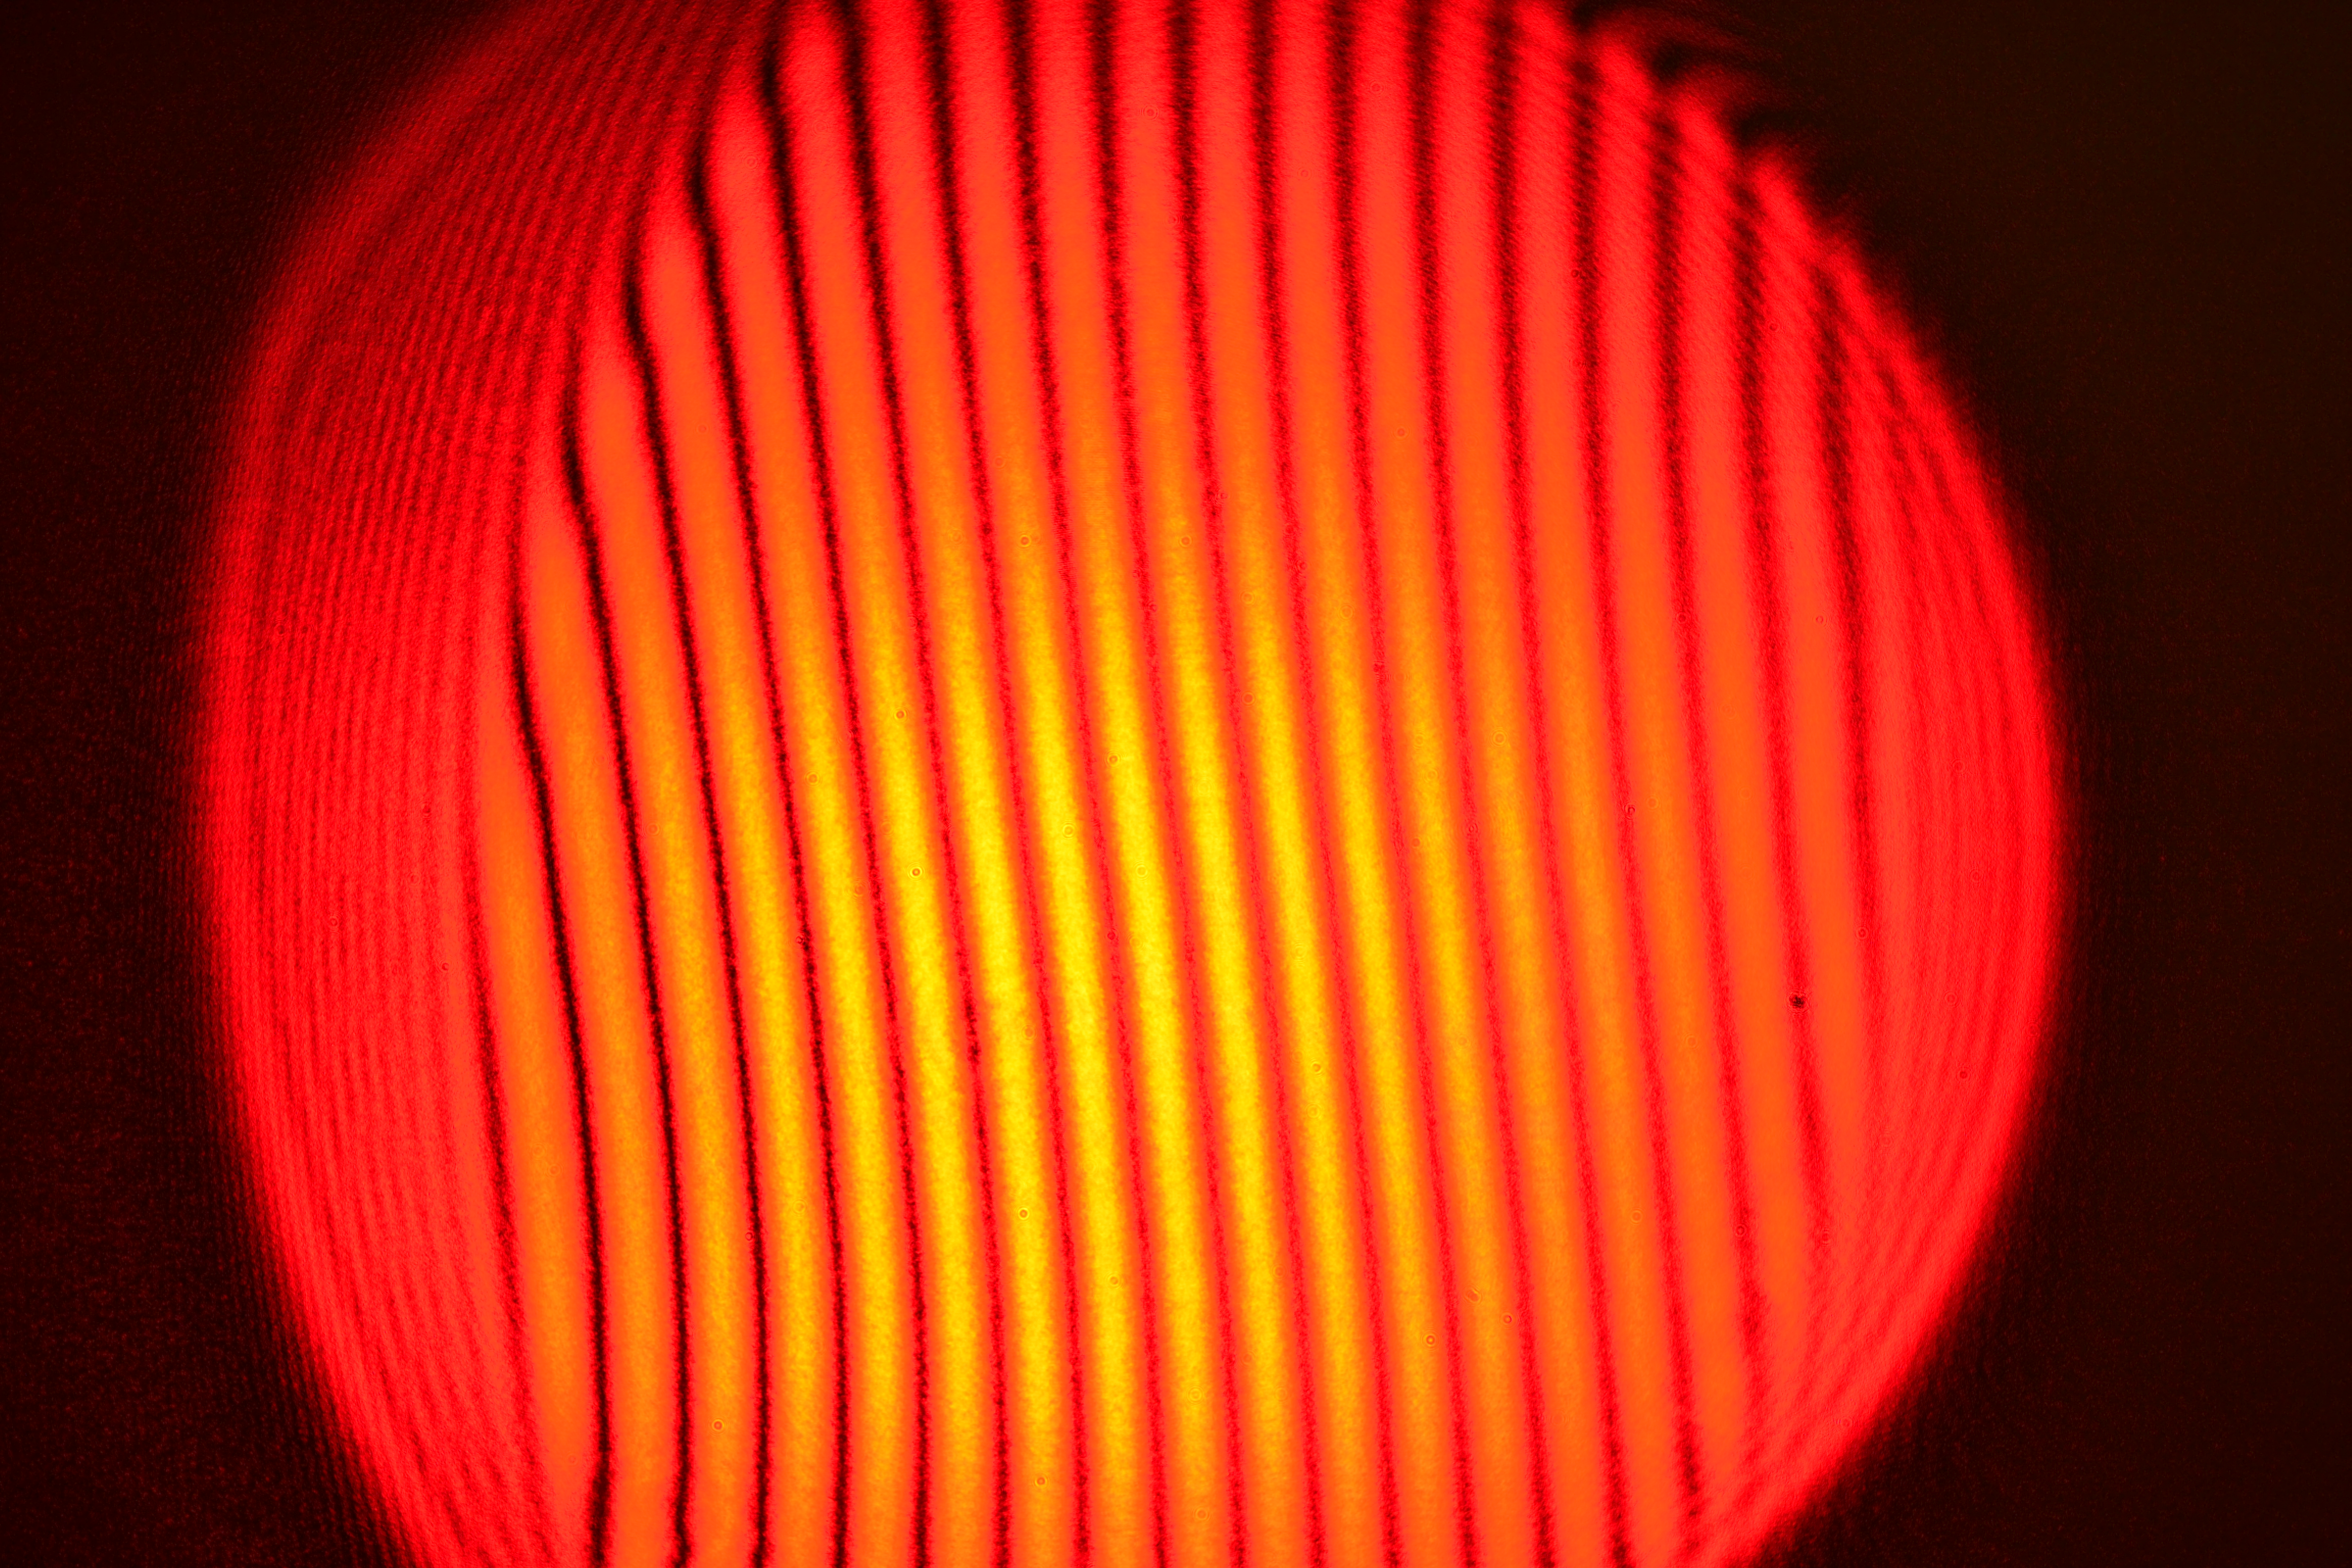
\includegraphics[width=.20 \textwidth]{Figures/Figures_I/DSC_0001.JPG}\hfill
    \includegraphics[width=.20\textwidth]{Figures/Figures_I/Tampered_MZ.png}\hfill
    \caption{Reference vs Tampered interference patterns observed by the camera.}
    \label{fig:Tampered_MZ}
\end{figure}

Later we proceeded to test the interference under different conditions. First, we introduced a flame to one of the paths. When we apply a flame to one of the interferometers arms, the fringes seem to amplify ,deform and loose contrast. This can be explained because light from a flame is not polarized. Hence most of the light does not interfere with the beams and we observe low contrast because we introduced some background light. Deformation can be explained because the density of air is compromised by the flame and this introduces a change in the optical path of one of the beams. This changes the phase of the resulting wave and becomes this visible effect illustrated in figure \ref{fig:FlameMZ}.  

\begin{figure}[H]
    \centering
    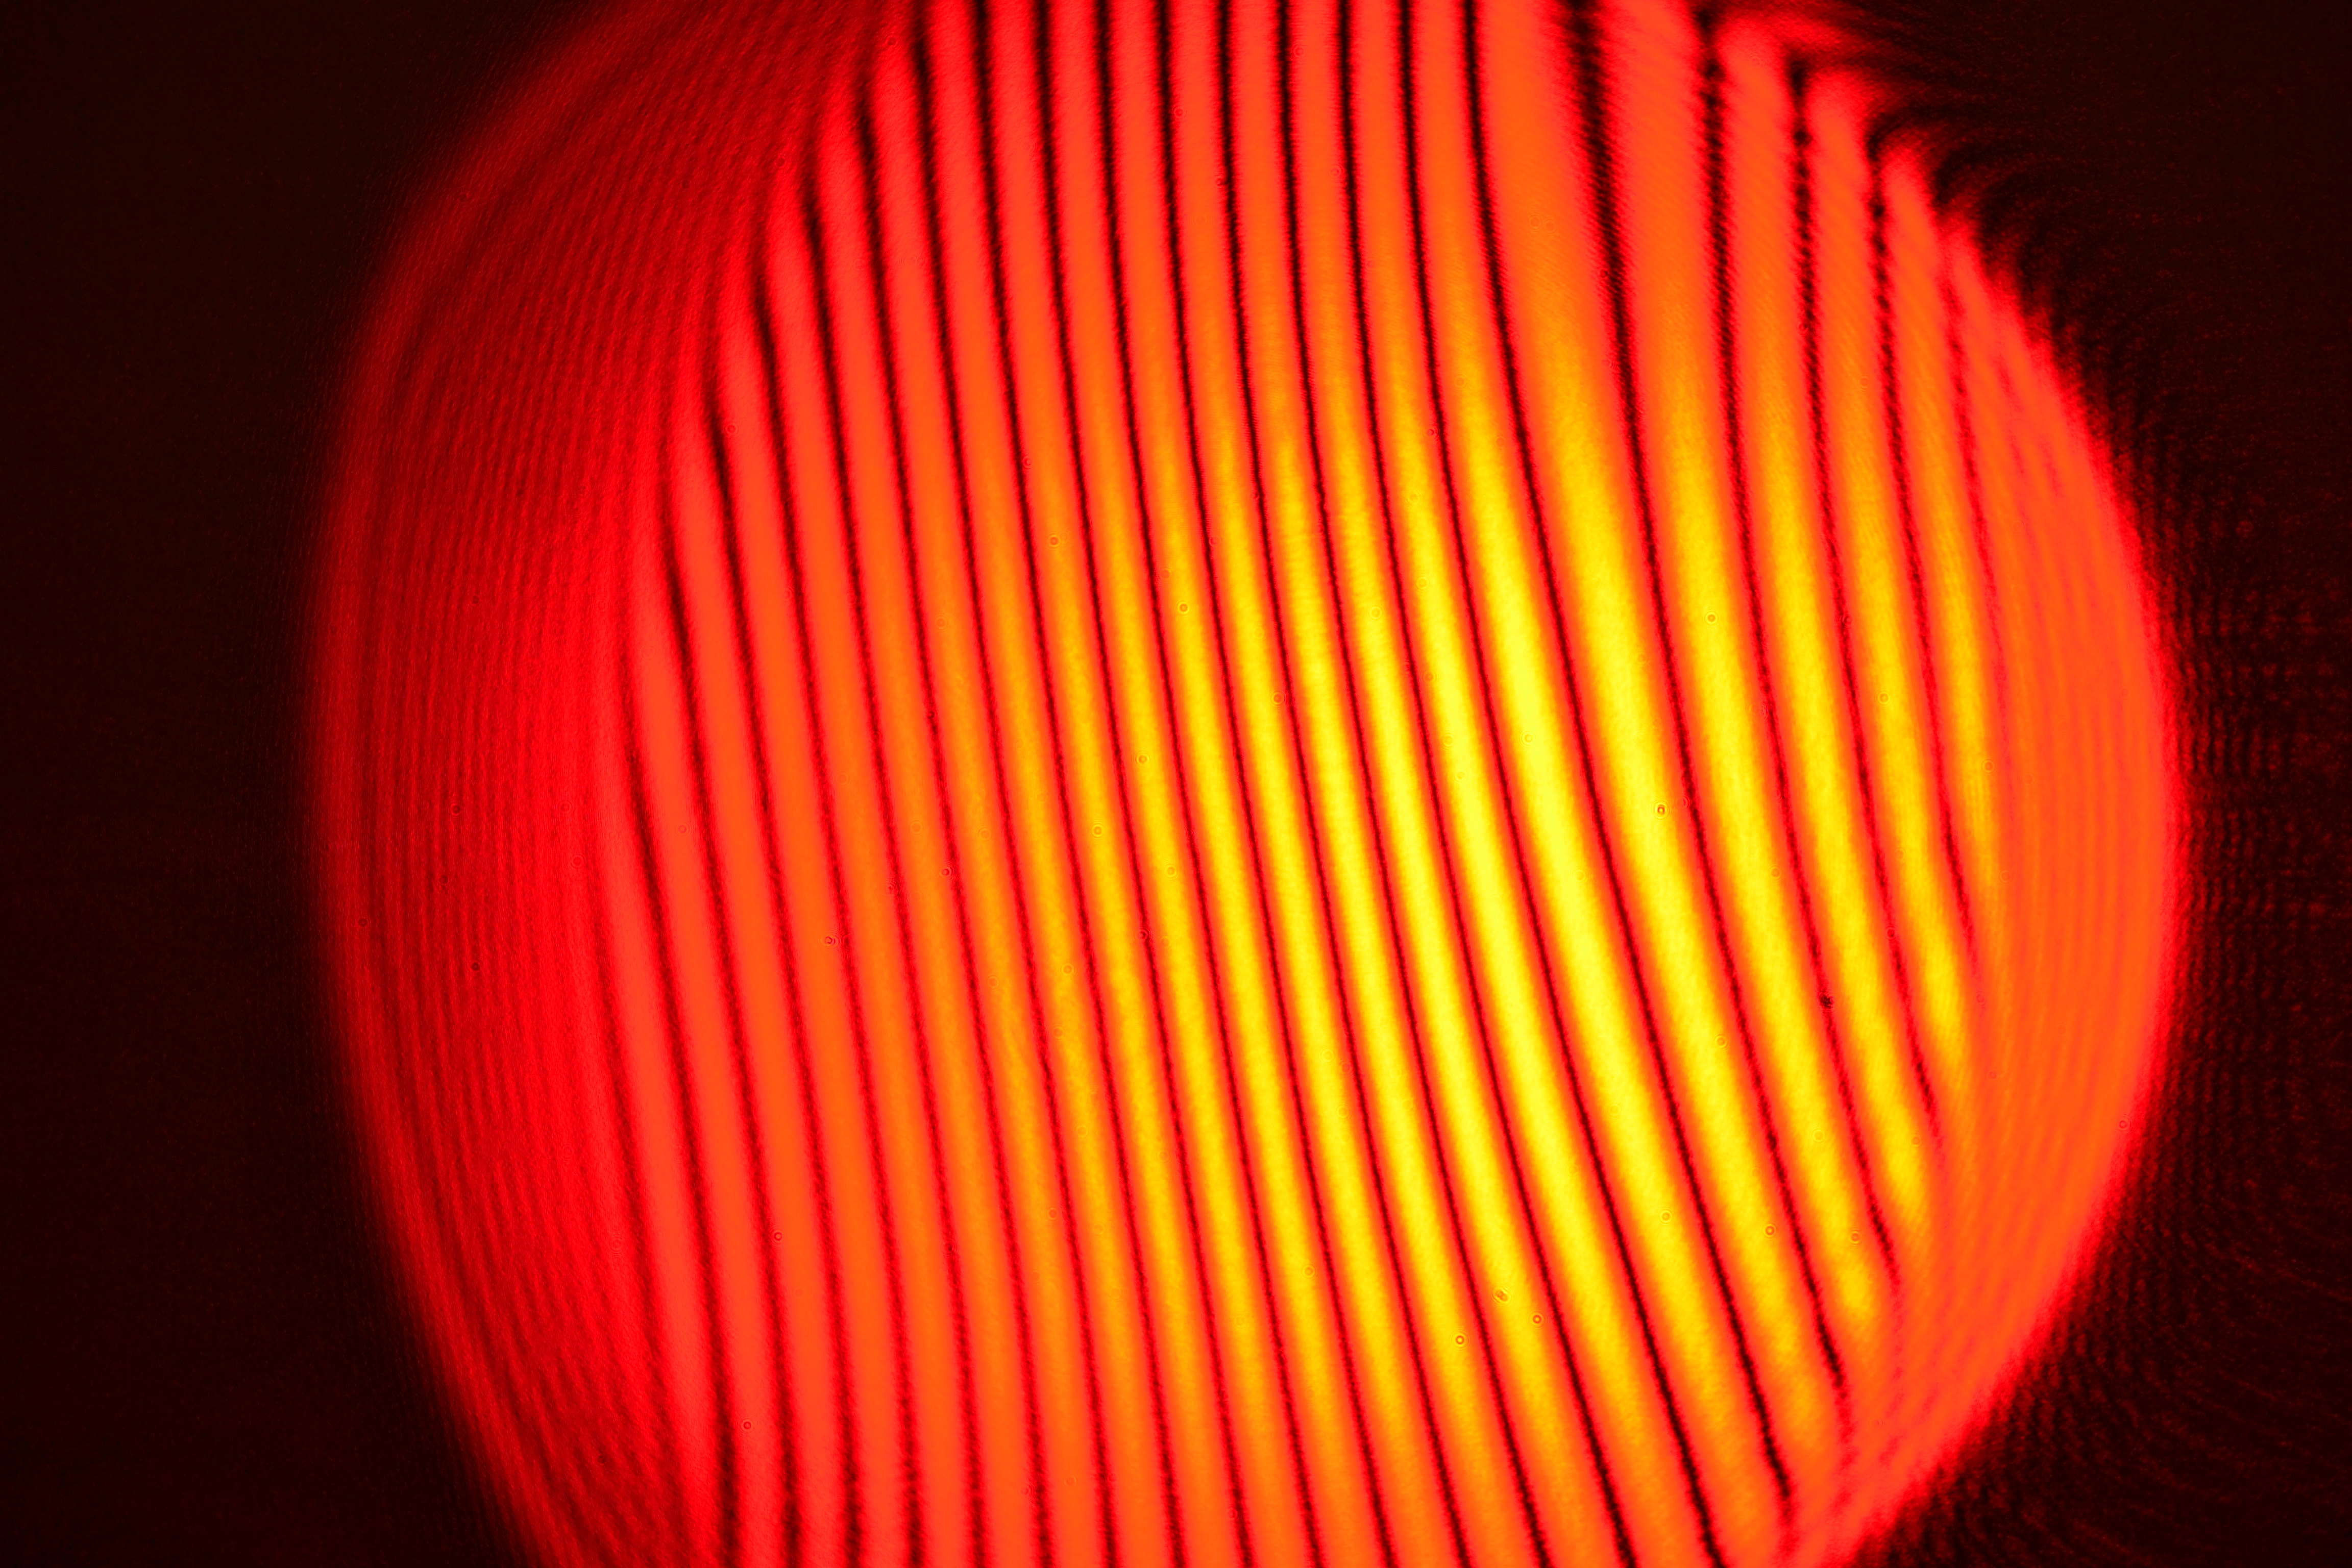
\includegraphics[scale=0.09]{Figures/Figures_I/Flame_MZ.JPG}
    \label{fig:FlameMZ}
    \caption{One of the arms is introduced a flame.}
\end{figure}

Minor alterations on the mirrors drastically affect the system. By moving the orientations \footnote{In the order of millimeters} of the mirrors in one of the arms we can introduce a variation in the angles between the vectors of propagation $\vec{k_1} $ and $\vec{k_2}$ corresponding to the two interfering beams. This leads to more or less fringes -and their orientation- in the interference patterns. 

\begin{figure} [H]
    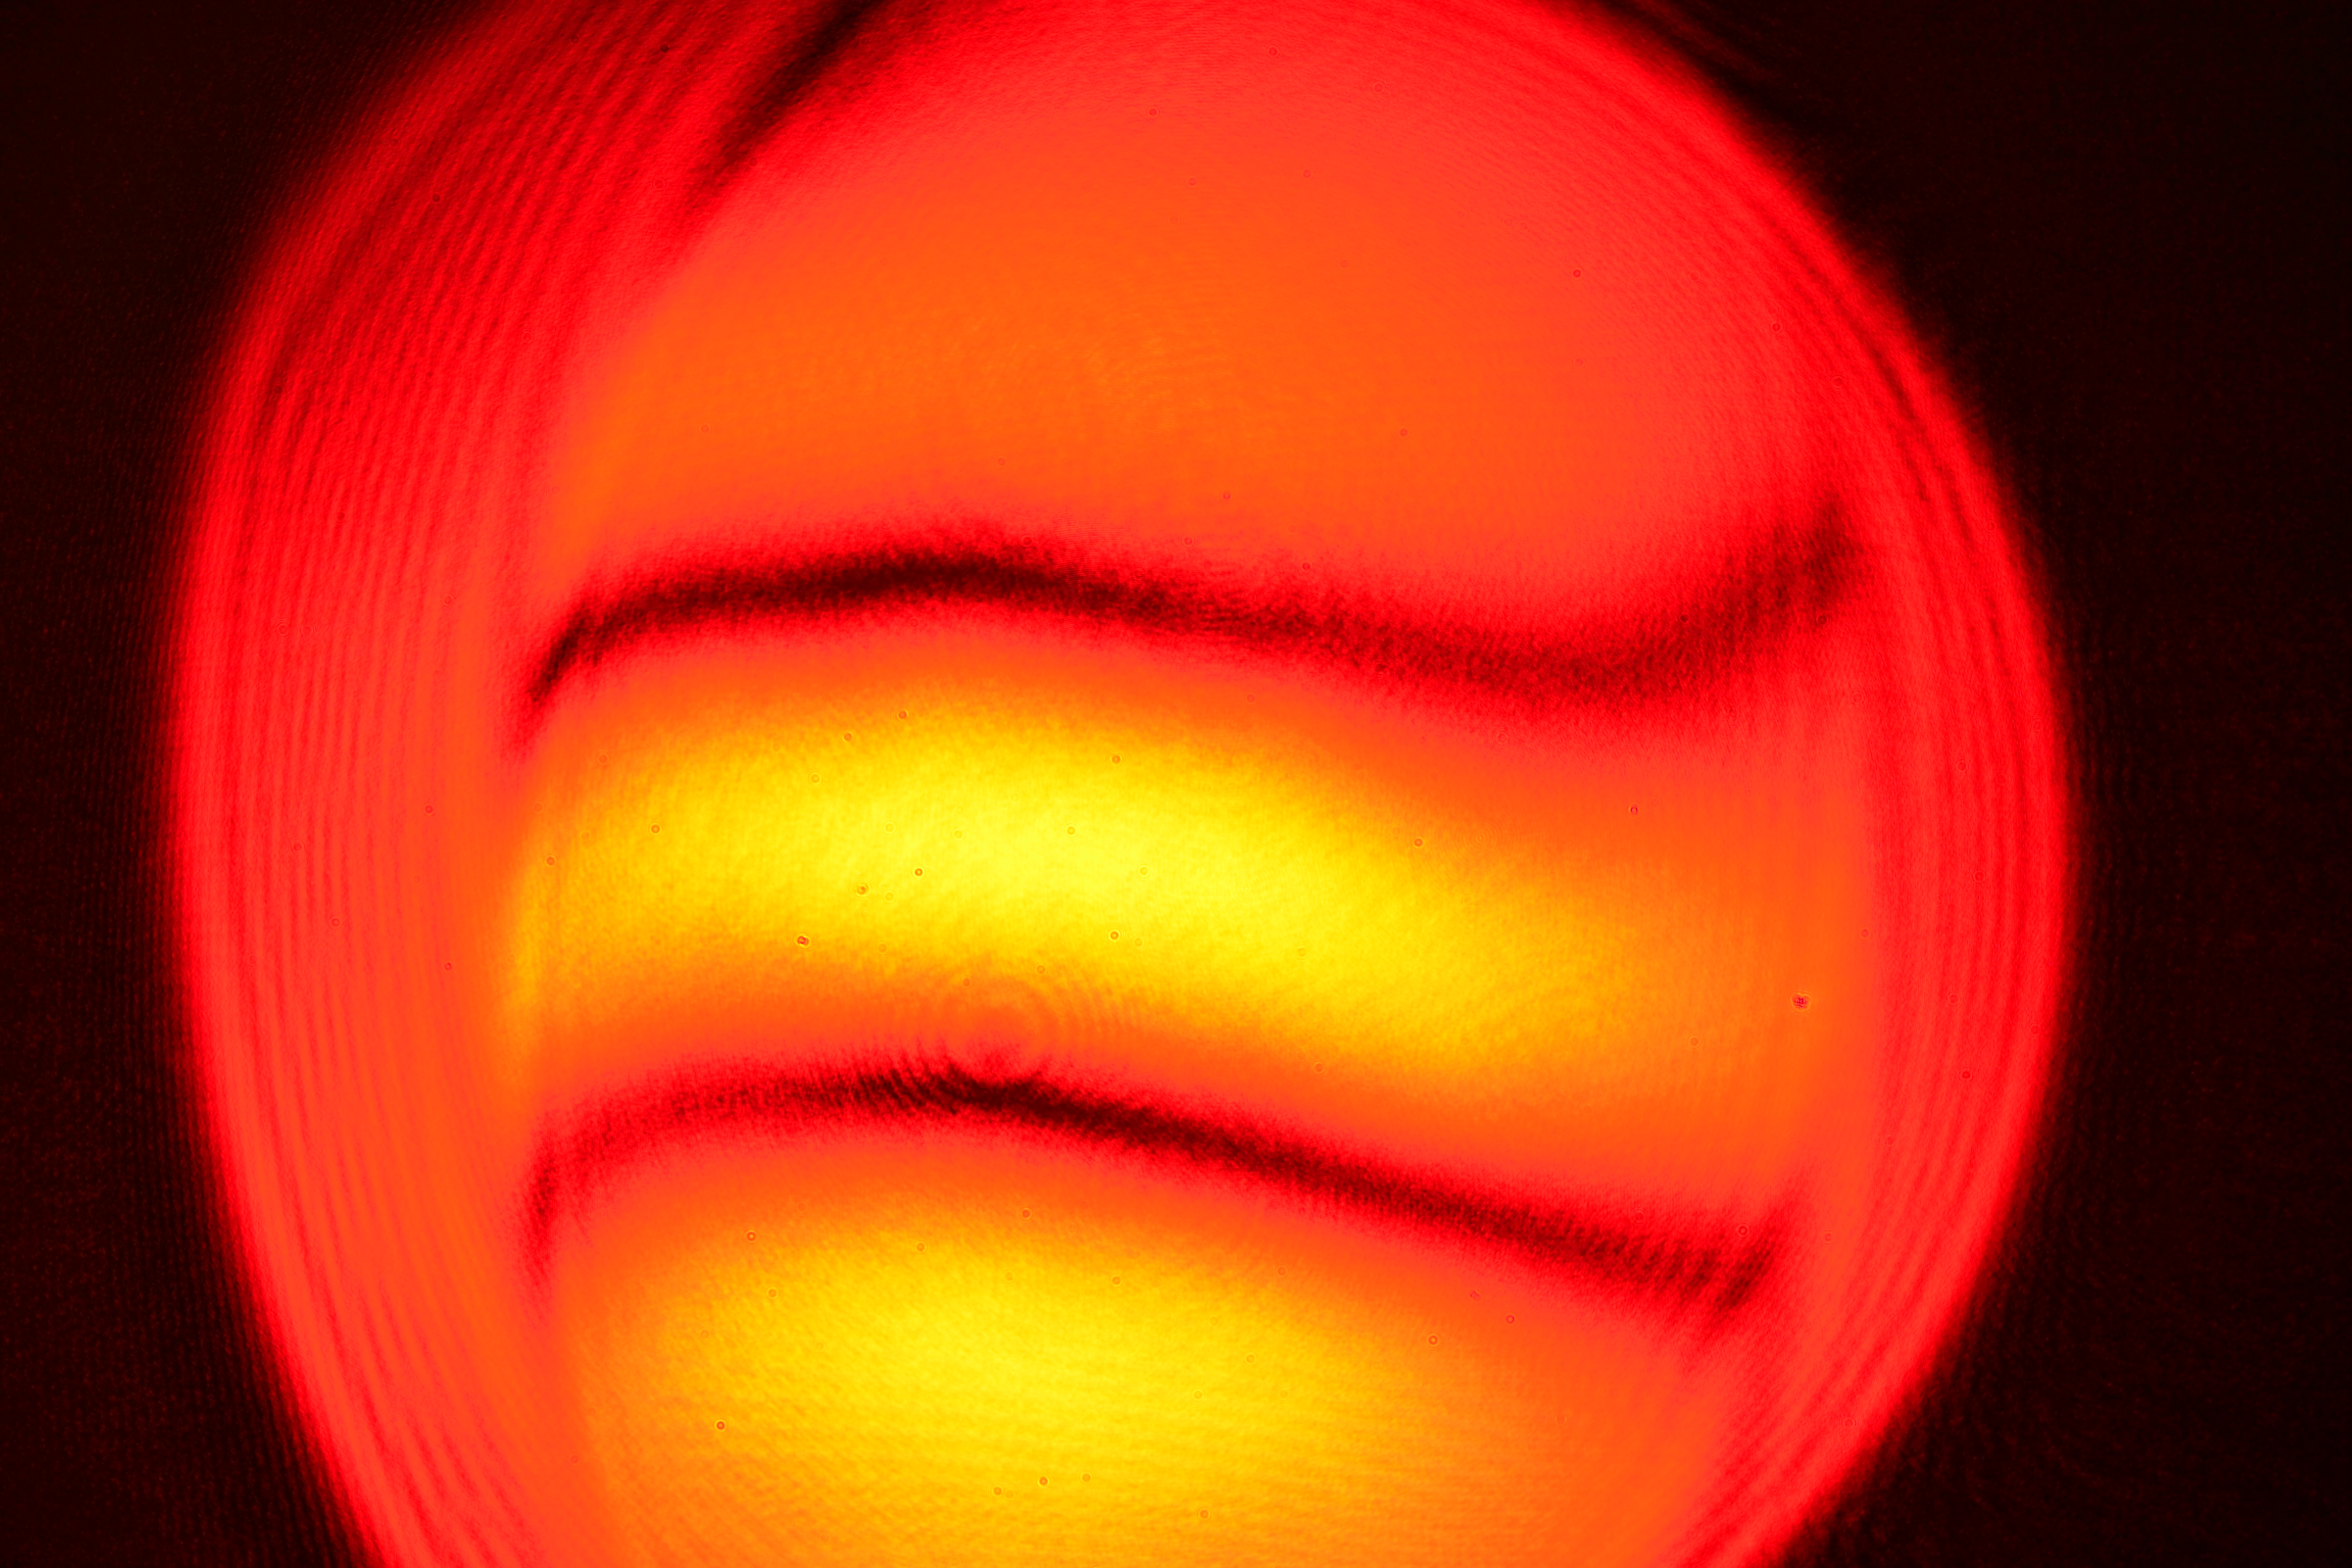
\includegraphics[width=.20 \textwidth]{Figures/Figures_I/Mirror_Movment1.JPG}\hfill
    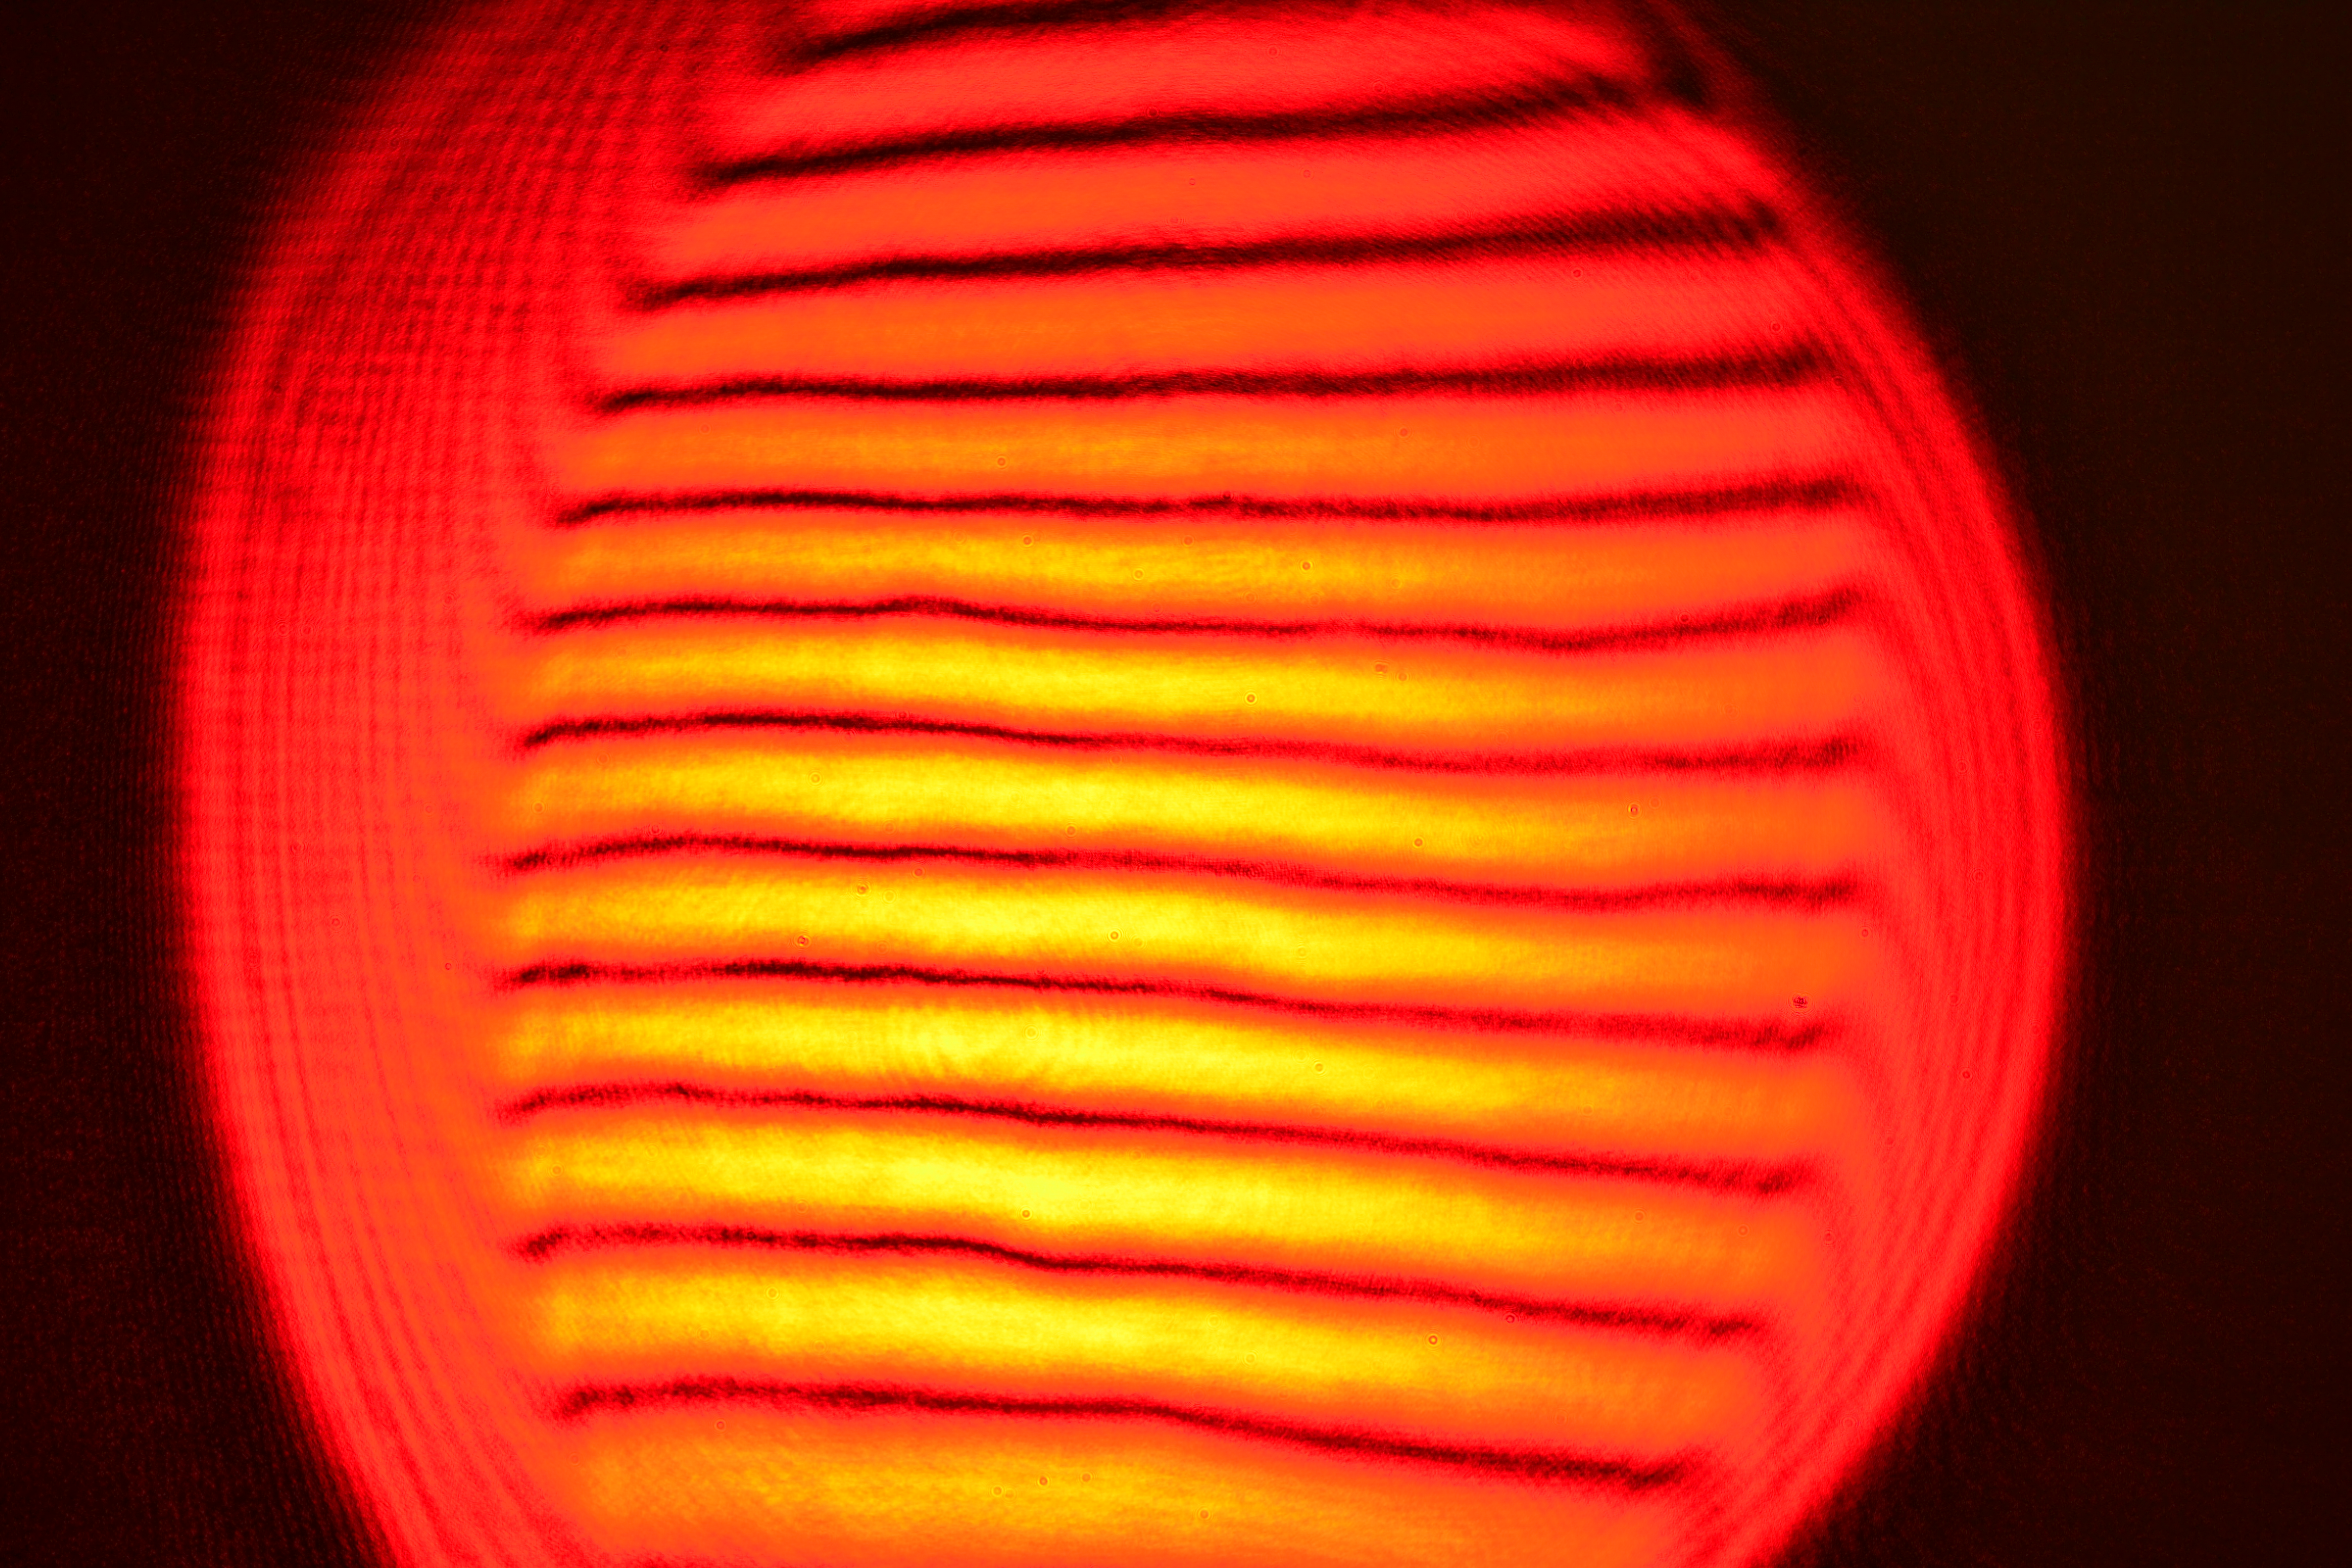
\includegraphics[width=.20\textwidth]{Figures/Figures_I/Mirror_Movment2.JPG}\hfill
    \caption{Interference patterns by phase difference observed by the camera.}
    \label{fig:kvectors}
\end{figure}

Another important observation is when the team introduced a intensity filter (0.5 ND) along one of the Mach Zehnder´s arms (Position 2). As shown in figure \ref{fig:filters}, the contrast of the fringes decreases notably.  This is due because the filter absorbs intensity that would otherwise be interfering with the other beam. Therefore, taking as a reference figure \ref{fig:filters} A; we can observe a difference in contrast. With the filter configuration, the fringes show a lower contrast. 

\begin{figure} [H]
    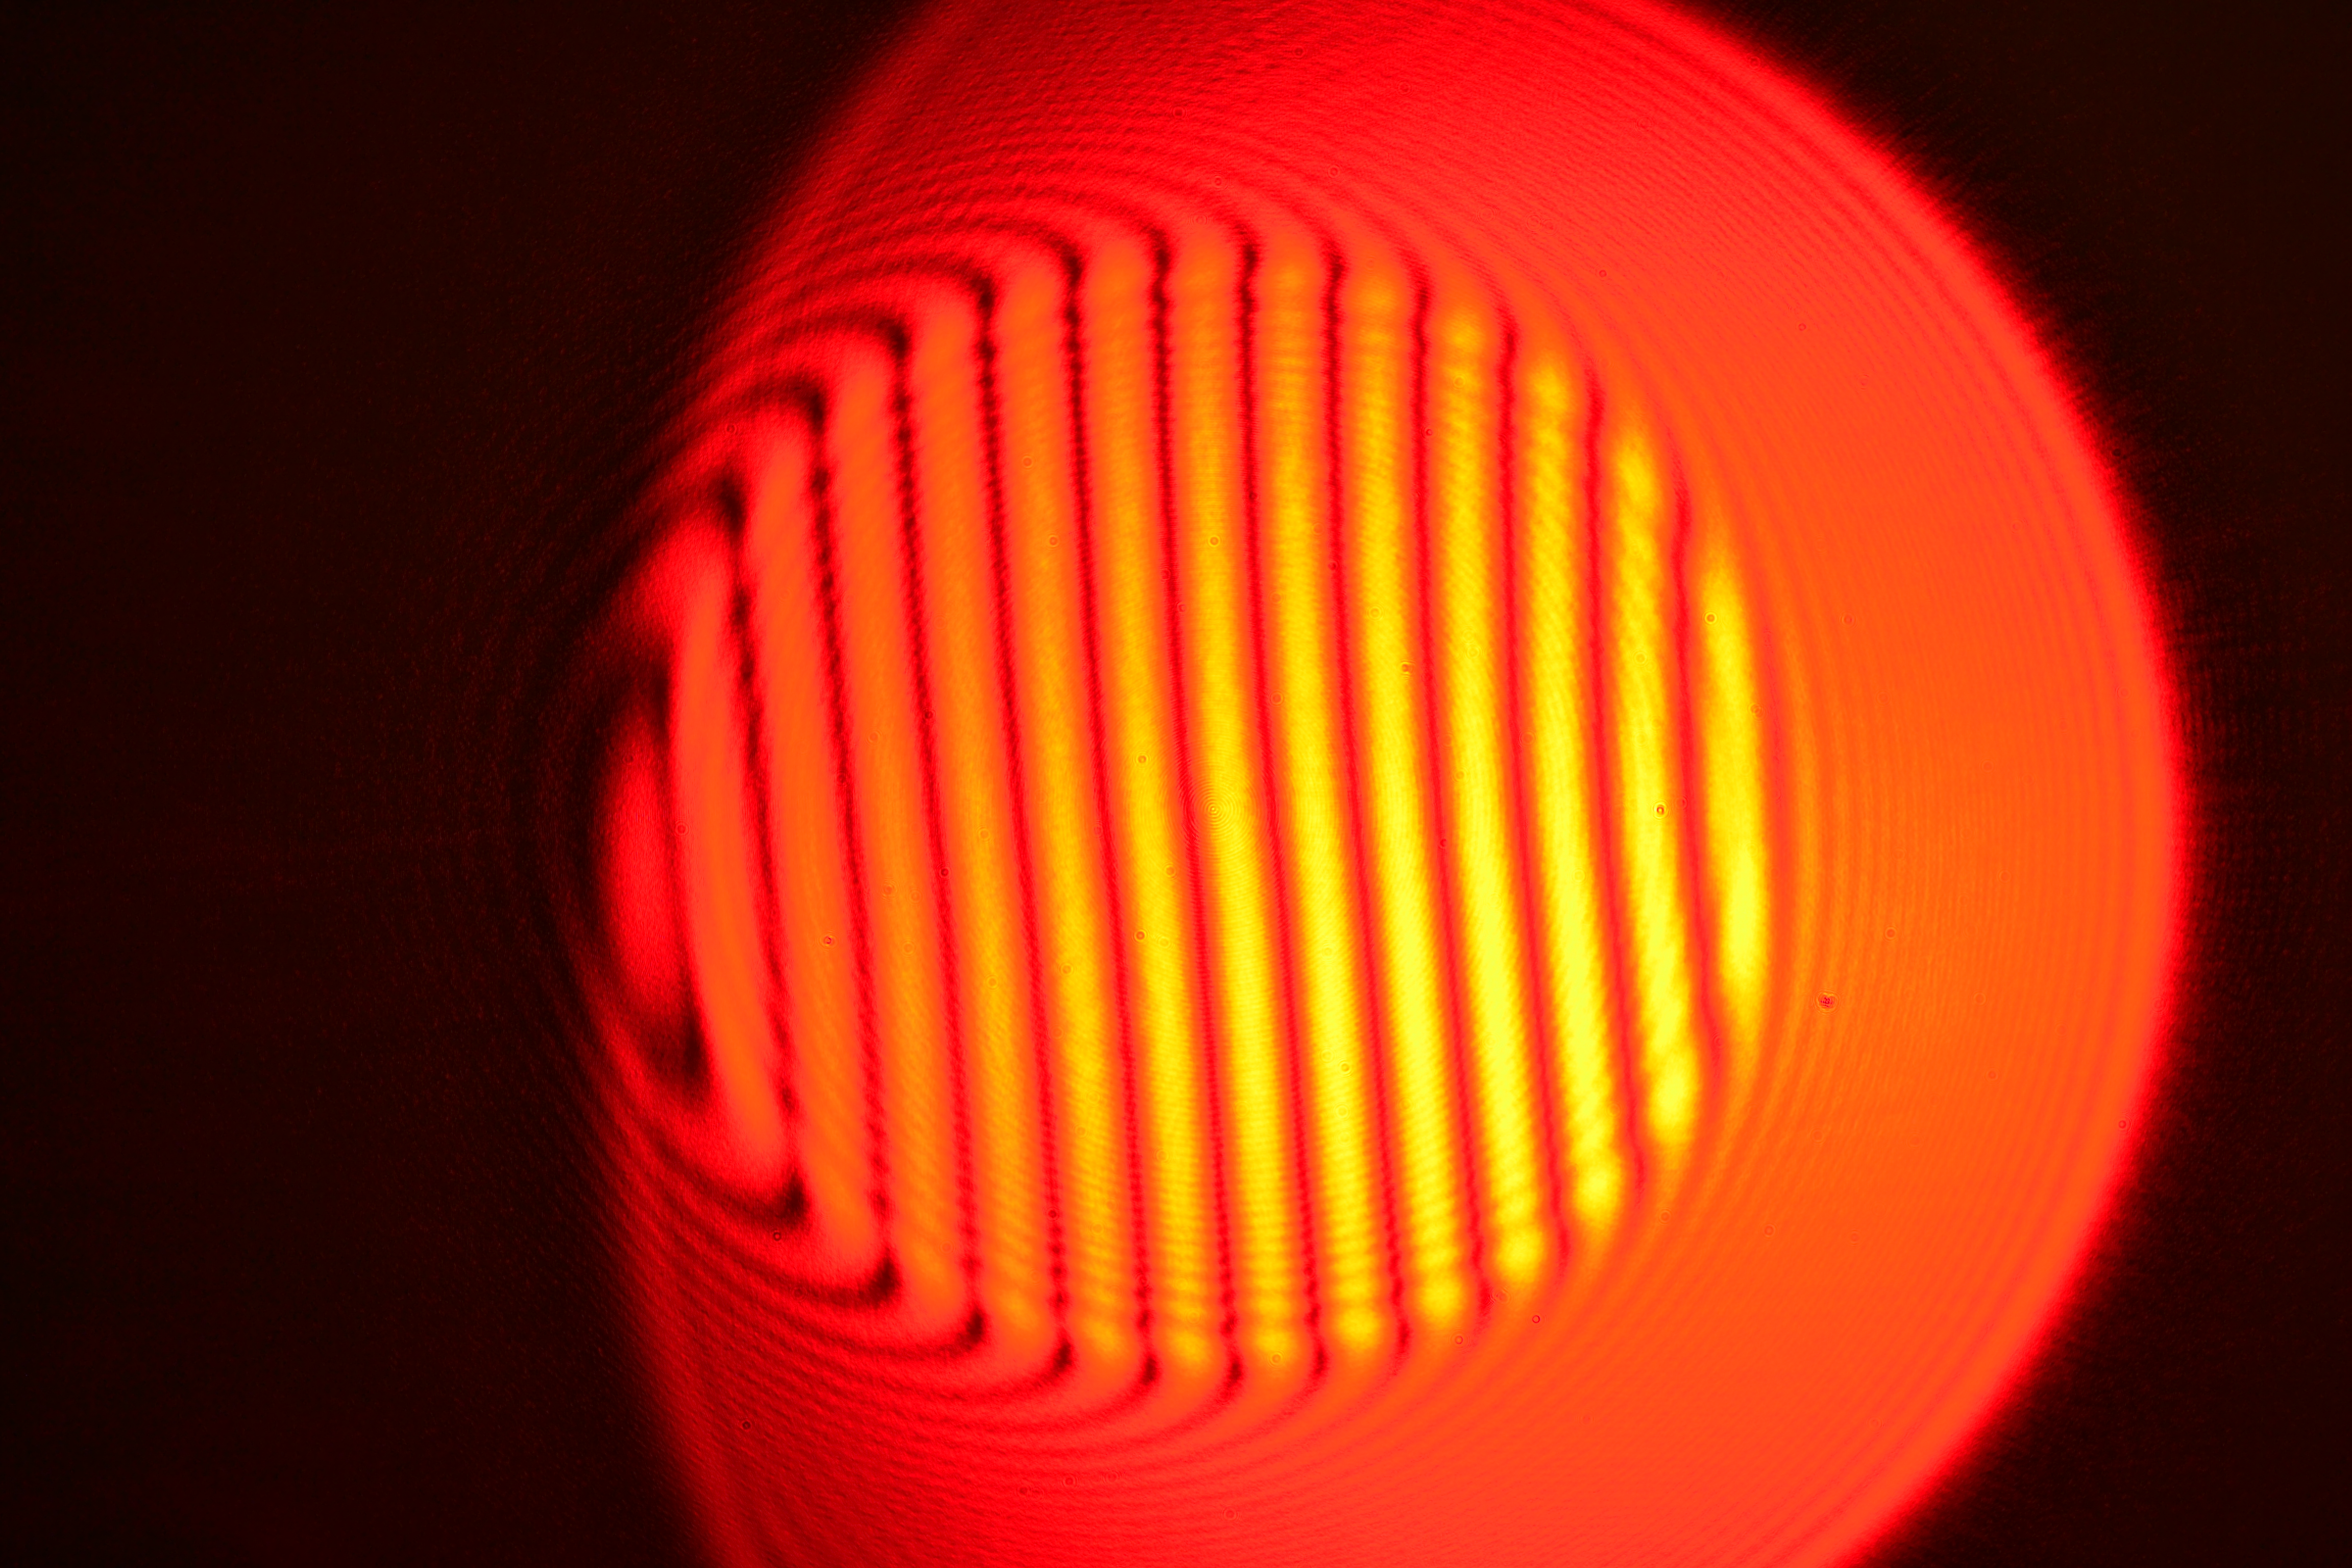
\includegraphics[width=.20 \textwidth]{Figures/Figures_I/MZ_Filter0.3.JPG}\hfill
    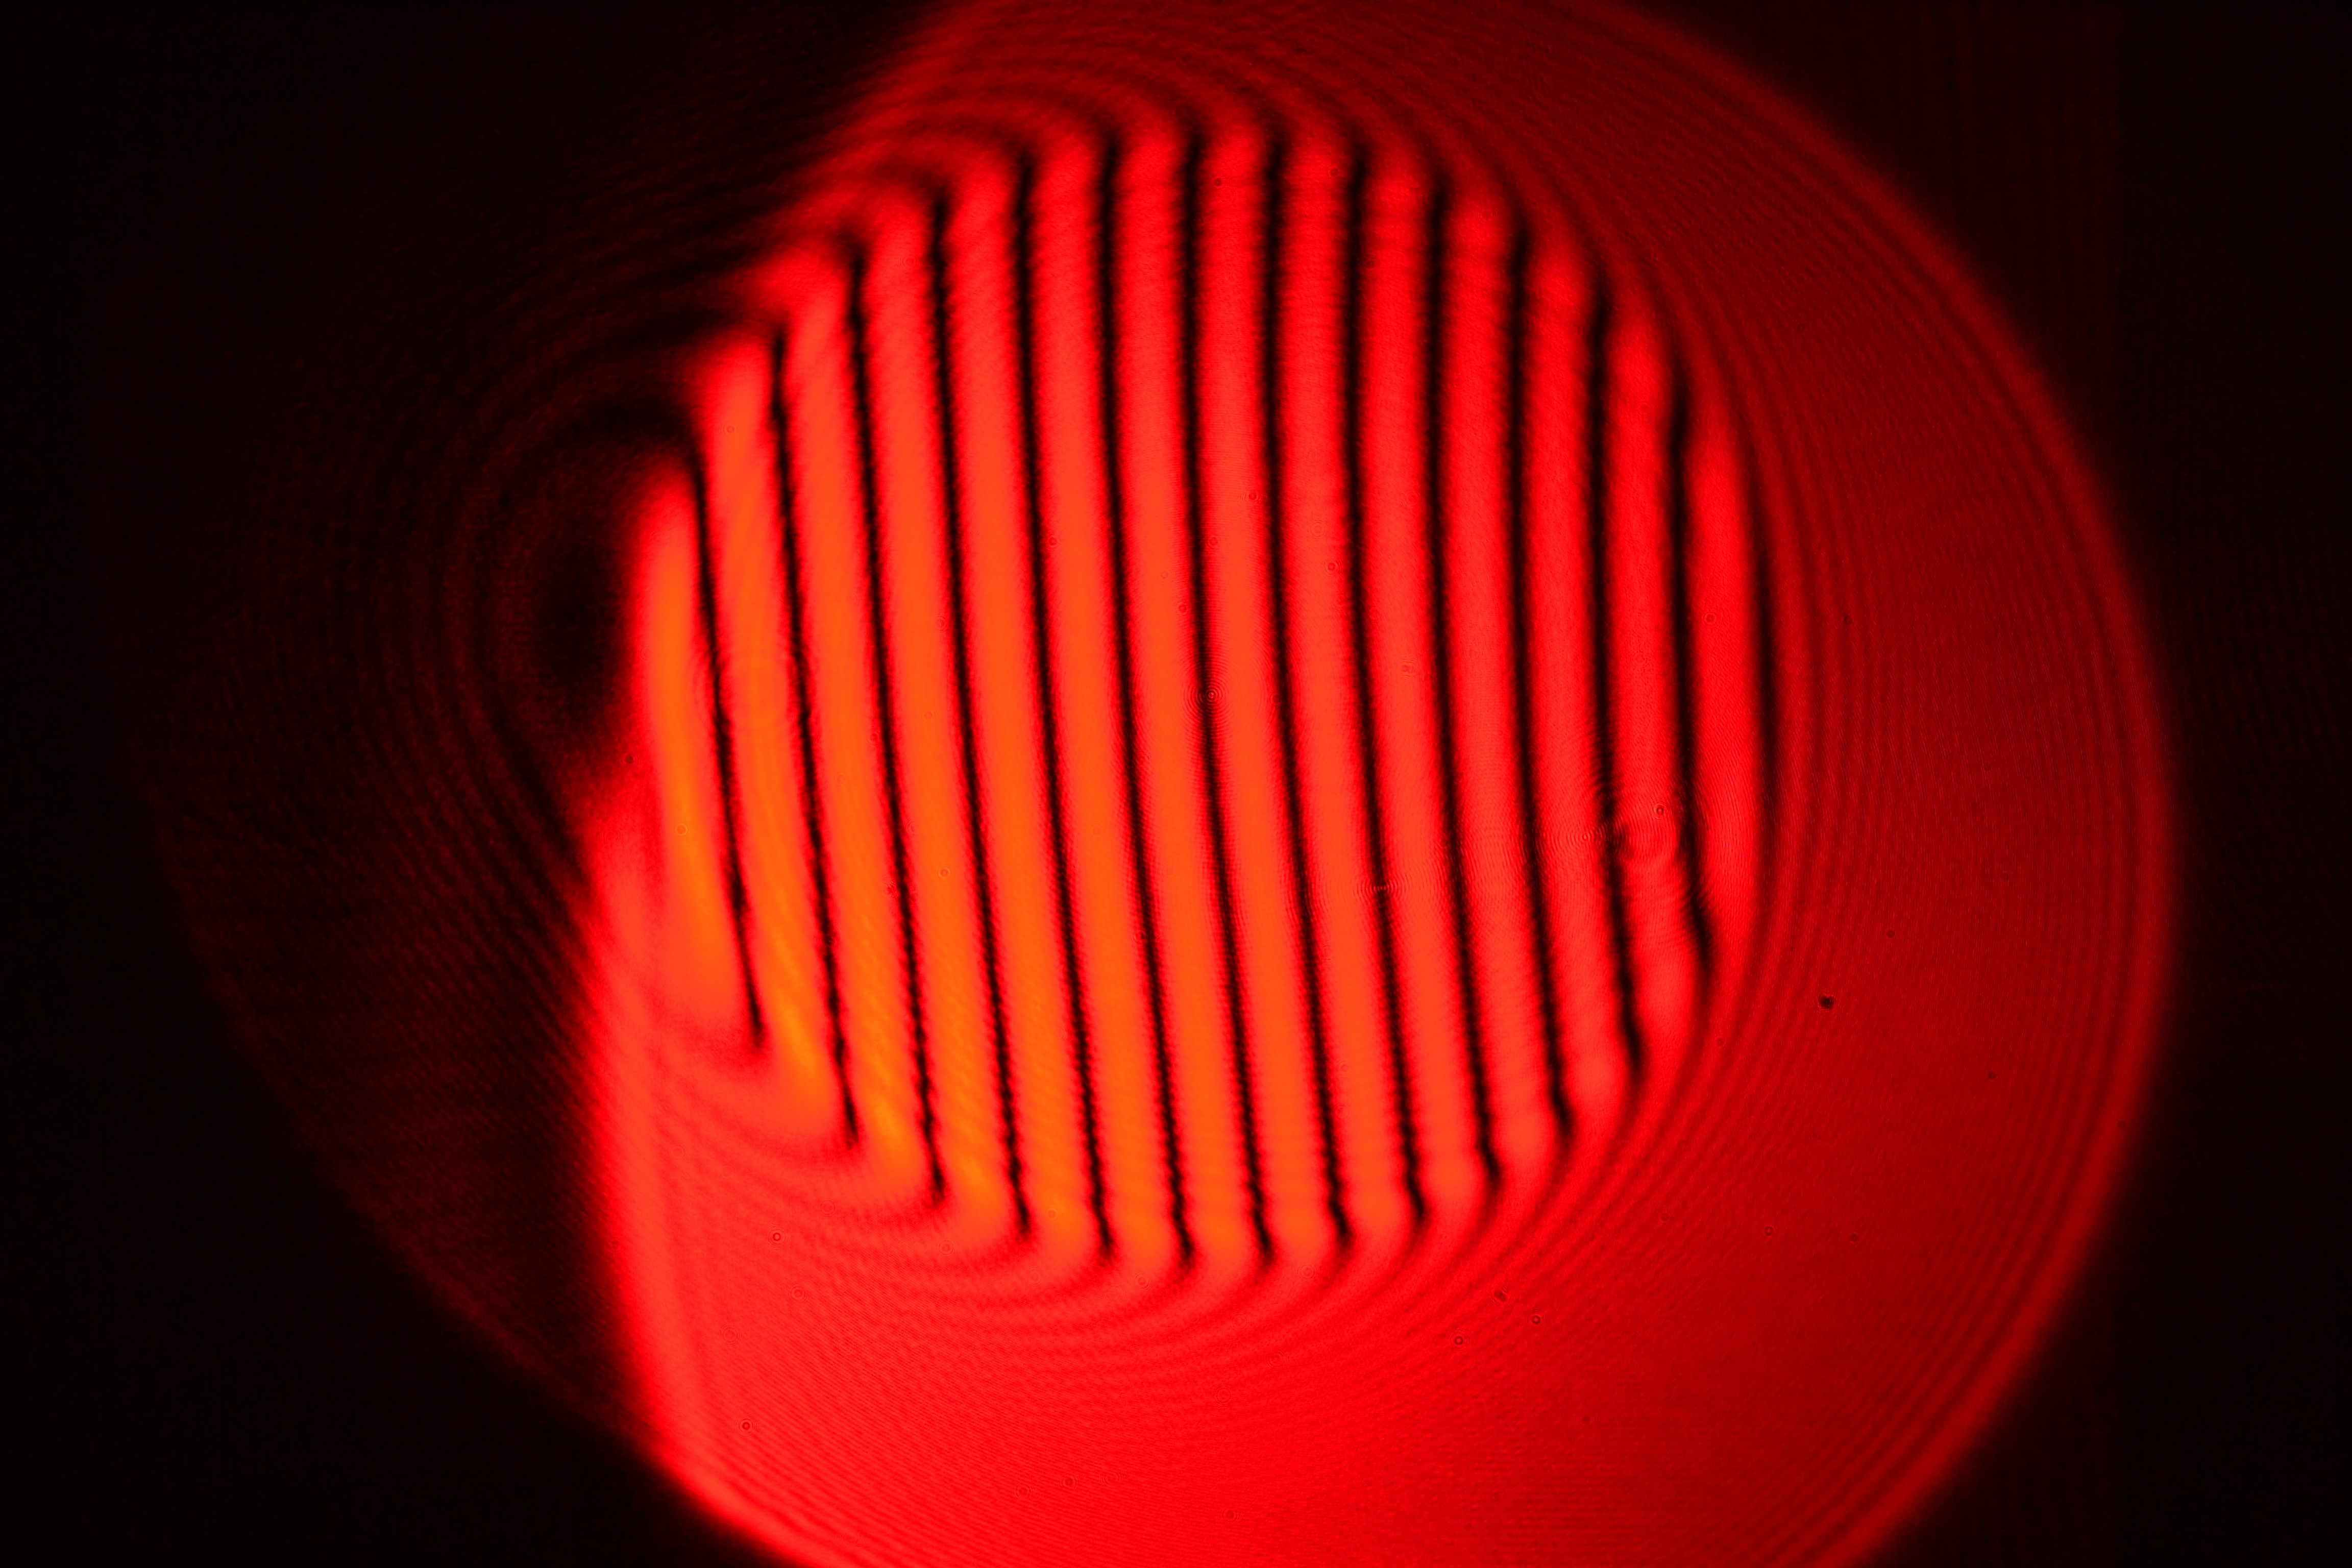
\includegraphics[width=.20\textwidth]{Figures/Figures_I/MZ_NoFilter.JPG}\hfill
    \caption{Filtered vs Non Filtered interference patterns observed by the camera.}
    \label{fig:filters}
\end{figure}

\subsection{POLARIZATION EFFECTS}

In section \ref{sec:TEO_FRAMEWORK} we discussed that a shared state of polarization is needed in order to interference to emerge. To test this statement empirically, we introduced in position 3 (Figure \ref{fig:Setup_MZ}) a half wavelength $\lambda /2$ retarder at a $45 ^o $ degree angle from its fast axis which in turn matches the orientation of the polarized state of the beam. This inverts the polarization on the beam by $90 ^o $ degree. At this point (Figure \ref{fig:polMZ} A), the two beams do not form interference because the polarization states are perpendicular to each other. Then the team adjusted the angle of the $\lambda /2$ retarder to $0 ^o $ -I.e not affecting the initial polarization state - we observe the interference pattern once again (Figure \ref{fig:polMZ} B). The team later proceeds to introduce the two perpendicular polarization states until the interference fringes disappear. To recover the interference patterns once again, we first mounted a linear polarizer in position 4. By aligning the polarizer to a $45 ^o $ degree angle from the vertical state of the LASER we observed the fringes once again (Figure \ref{fig:polMZ} C)! This is because the interfering vertical and horizontal states can be thought of a superposition of a diagonal and anti diagonal states. In linear algebra this is known as a chance of basis. Thus, the diagonal polarizer in position 4 allows both beams to interfere in its diagonal polarization state and the observation leads to fringes. 

\begin{figure} [H]
    \includegraphics[width=.14 \textwidth]{Figures/Figures_I/MZ_Fringes (3).JPG}\hfill
    \includegraphics[width=.13\textwidth]{Figures/Figures_I/MZ_Fringes (4).JPG}\hfill
    \includegraphics[width=.17\textwidth]{Figures/Figures_I/MZ_Fringes (5).JPG}\hfill
    \caption{A) No interference because of perpendicular polarization states. B) Interference because 2 parallel polarization states. C) Interference because perpendicular states interfere in a diagonal polarized orientation. }
    \label{fig:polMZ}
\end{figure}


\subsection{PHASE RETARDATION BY $\Delta \Lambda$}
In the previous subsection the team found that introducing a different air density -due to the presence of a flame- in one of the interferometers arms leads to different interference patterns. This is because a difference in the optical path $\Delta \Lambda$ is introduced and the beams interfere with each other at different phases. To test this phenomena in a more controlled matter, the team proceeded to introduce a glass plate in position 2 (Figure \ref{fig:Setup_MZ}). This made one of the beams refract and thus introducing a $\Delta \Lambda$. Figure \ref{fig:GlassSetup} is a picture of the visible interference affected by the glass (white borders) and the unaffected by the glass on the bottom of the picture.
\begin{figure}[H]
    \centering
    \includegraphics[scale=0.20]{Figures/Figures_I/GlassOneArm_MZ.png}
    \caption{Glass applied to half of a beam in position 2 at an angle.}
    \label{fig:GlassSetup}
\end{figure}
Two facts are very clear from figure \ref{fig:GlassSetup}: 1) the refraction angle caused by the glass shifts the vector of propagation in one of the beams and thus generates different number of fringes and 2) different orientations. 

\subsection{INTERFERING WAVE FRONTS}
Finally the team set up a configuration to study the interference of two different types of wave-fronts: plane waves and spherical waves. To achieve this, we introduced a lens on position 3 (Figure \ref{fig:Setup_MZ}). This focuses the incident plane (or collimated) wavefront generating a spherical wavefront. After this two wave-fronts interfere the following interference pattern emerges \cite{fig:Wavefronts}: 
\begin{figure}[H]
    \centering
    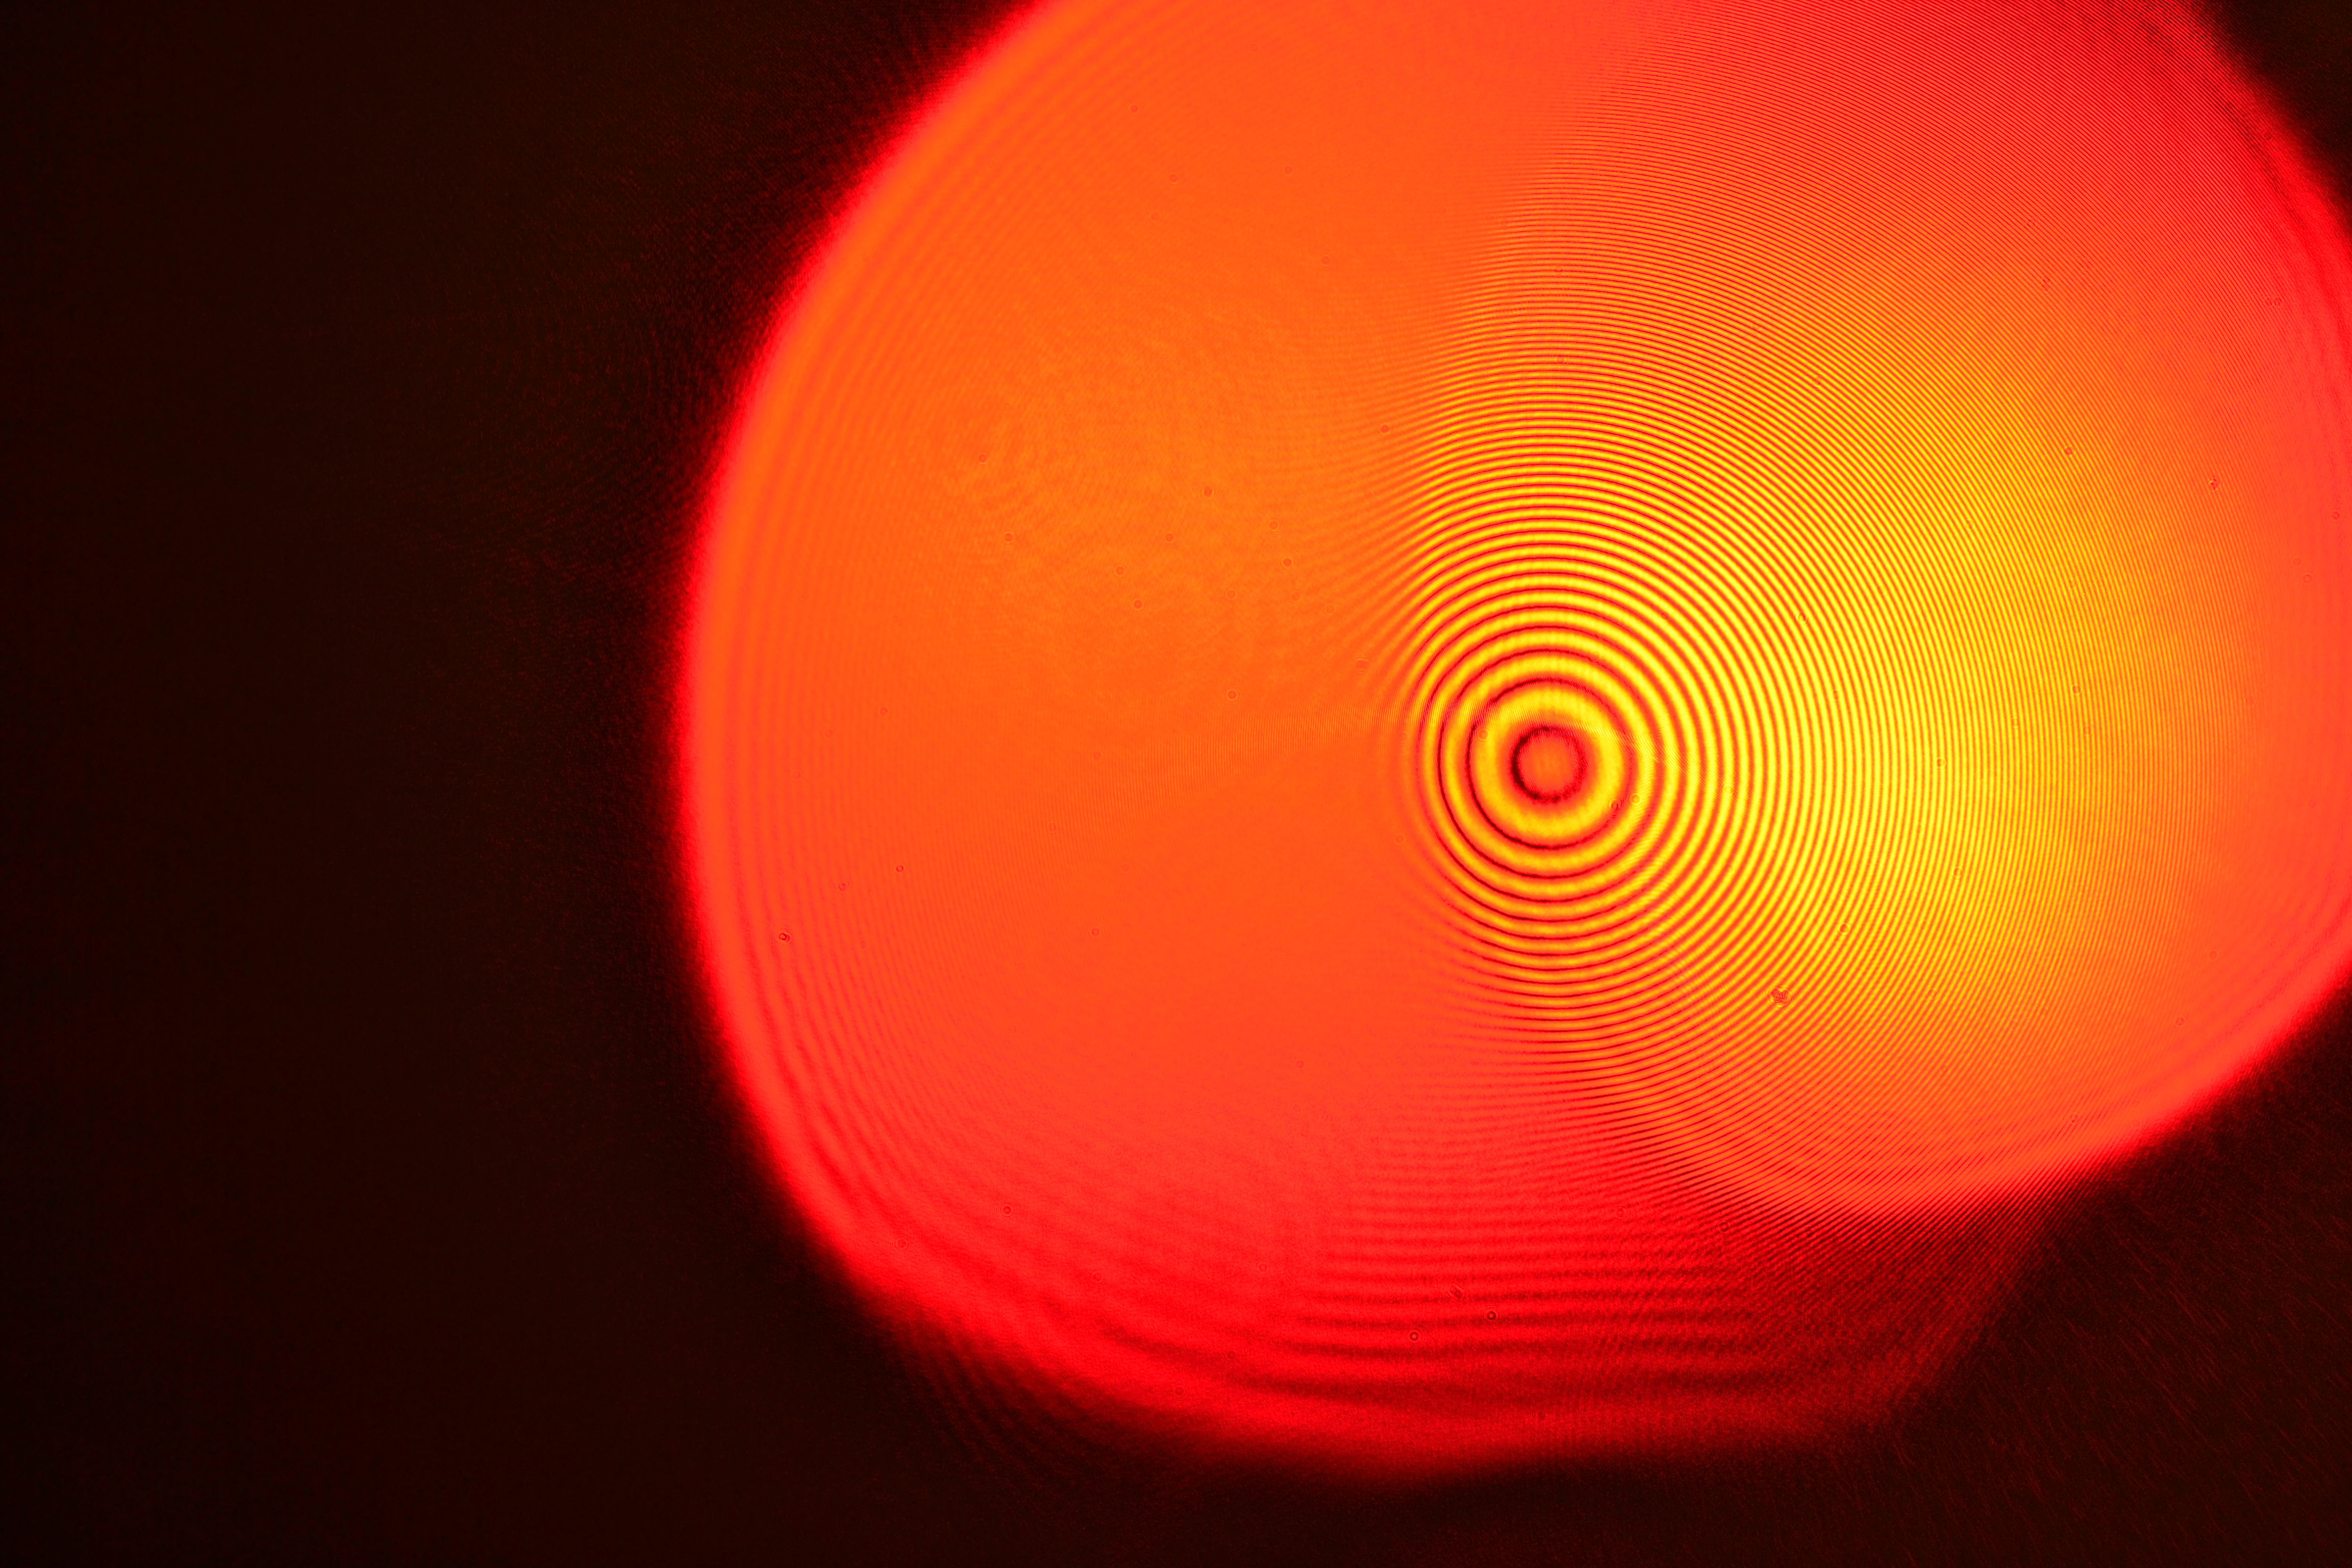
\includegraphics[scale=0.10]{Figures/Figures_I/Wavefronts_MZ.JPG}
    \caption{Plane and spherical interfering wave-fronts.}
    \label{fig:Wavefronts}
\end{figure}
The results are not good quality because of poor collimation techniques. However, during the experiment we observed that an array of concentric circles begins to form when these two wave-fronts interfere. 

\subsection{ALTERNATIVE INTERFEROMETERS BY PHASE DIVISION} 

Other configurations involving beam splitters include the Michelson and Sagnac configurations (Figure \ref{fig:MS}. They have other strong characteristics that can allow physicists to measure different characteristics of the interference phenomena. 

\begin{figure}[H]
    \centering
    \includegraphics[scale=0.33]{Figures/Figures_I/MichelsonSagnac.png}
    \caption{A) Michelson and B) Sagnac interferometer.}
    \label{fig:MS}
\end{figure}

We will use this space to answer what I consider 3 pertinent questions about the phenomena of interference. 
\begin{enumerate}
    \item What happens to the energy when we have destructive interference?
    \item What is the coherence of our LASER BEAM listed in section \ref{sec:mat}? 
    %\item What are the conditions to generate a wavefront with multiple polarization distributions? 
\end{enumerate}

The Sagnac interferometer was used by the team to measure the distribution of energy in the beam. The team built the configuration illustrated in figure \ref{fig:MS}, later a series of pictures where taken in order to obtain different fringe numbers and registering as matrix digital measurements. The integral of this transversal measurement can be related to the energy as displayed in (Figure \ref{fig:SagResult}). Resolving question 1): In regions of destructive interference, energy is in a different configuration state but still conserved due to compensation in regions inside the constructive case.
\begin{figure}[H]
    \centering
    \includegraphics[scale=0.25]{Figures/Figures_I/SagnacResult_EnergyConservation.jpg}
    \caption{Energy conservation readings match up to value of $92\%$ of energy conservation. }
    \label{fig:SagResult}
\end{figure}

Michelson's interferometer its optimal for experiments involving displacements in mirror. Thus, this configuration will allow the team to perform measurements of the coherence of the LASER. The team began re calibrating the interferometer. Later, we proceeded to move the mirror such that $l_0 -> 0$ and stop when we no longer observe where the interference (Figure \ref{fig:MichRes}). The measured value was $x_{I0} =0.00 cm $. Later we varied $l_0 -> \inf$ because the nature of the LASER is not purely monochromatic, the coherence of the beam will hold for a finite range of distance values . We observed a distance where the fringes are no longer distinguishable. That distance is recorded as $x_{IF} =102.00 cm $. E.i the coherence distance ($\chi$) is 
\begin{equation} 
\chi = x_{IF} - x_{I0} = 102 cm, 
\end{equation} 
is related to the temporal coherence discussed in section \ref{sec:TEO_FRAMEWORK} by introducing the velocity (c)
\begin{equation} 
\tau = \chi / c [s]. 
\end{equation} 
Therefore after $\tau$ seconds, the LASER light decoheres. 
\begin{figure} [H]
    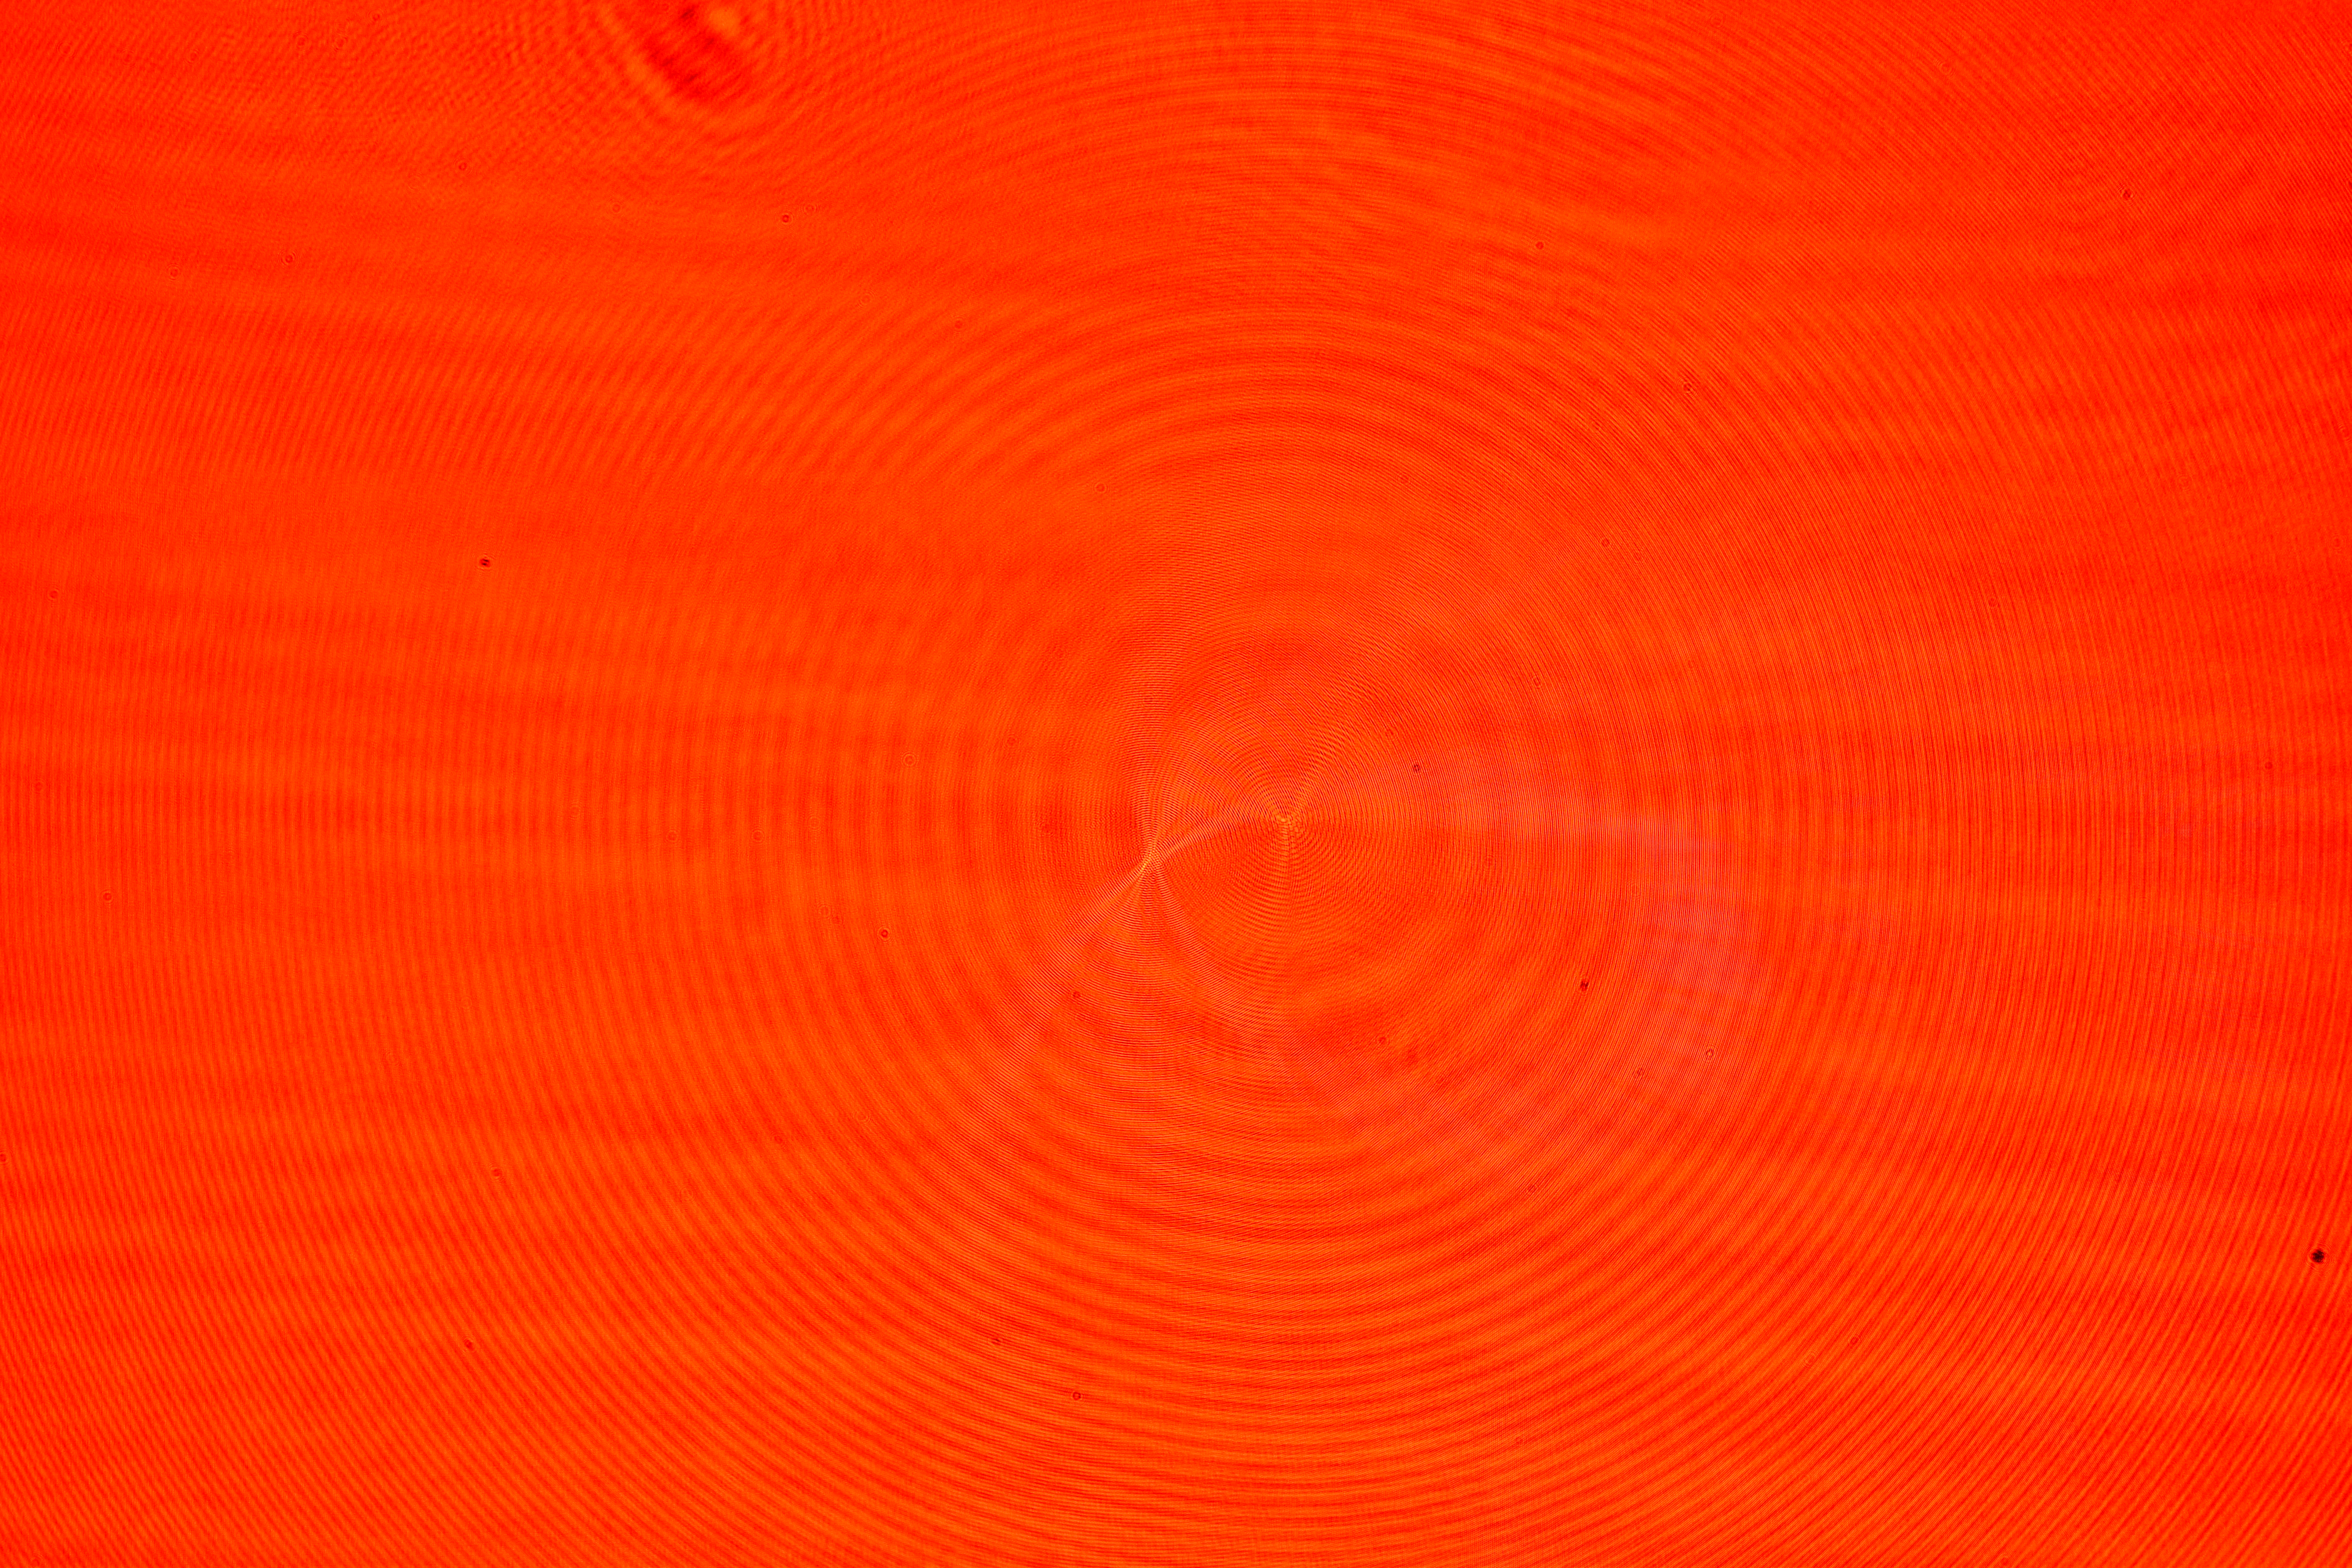
\includegraphics[width=.20 \textwidth]{Figures/Figures_I/DSC_0323.JPG}\hfill
    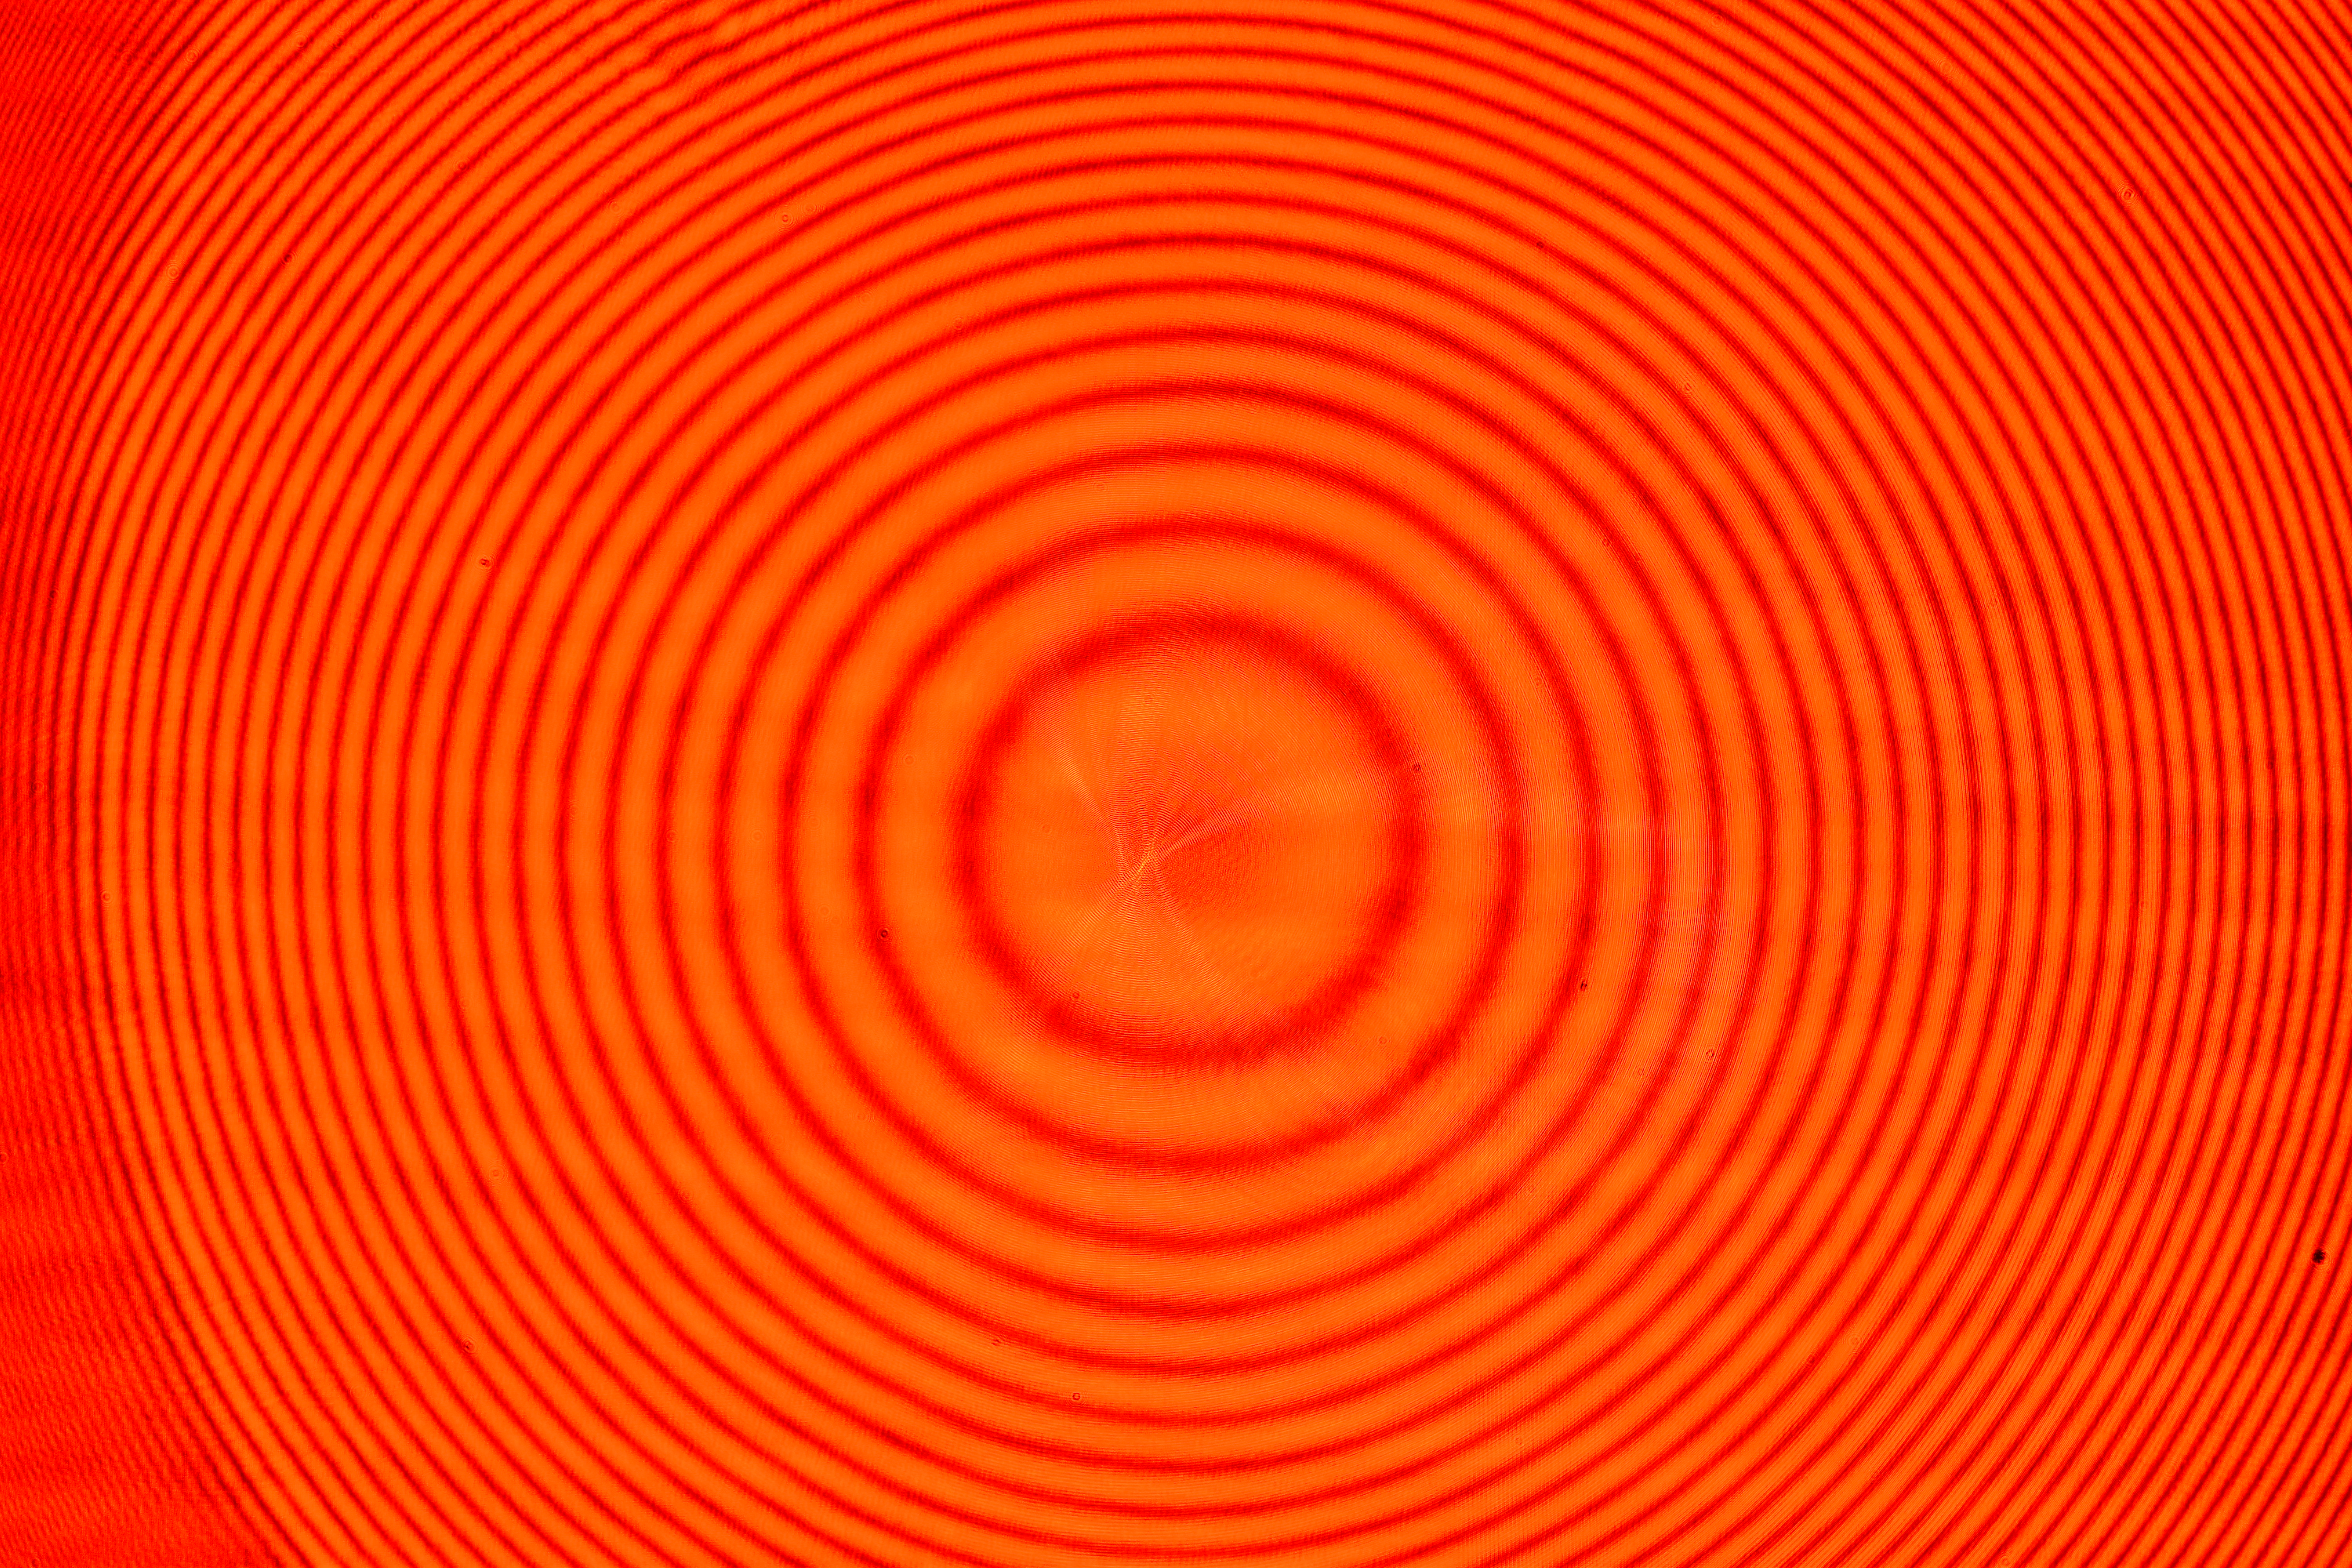
\includegraphics[width=.20\textwidth]{Figures/Figures_I/DSC_0321.JPG}\hfill
    \caption{$x_{IF}$ and $x_{I0}$ experimental results (respectively). }
    \label{fig:MichRes}
\end{figure}



%For the final part of this practice the team build Sagnac's Interferometer (Figure\ref{fig:MS}) with a polarized beam splitter \footnote{Where the reflected beam is horizontal and the transmitted beam is vertical.}. We measured stokes parameters to obtain wave fronts with different polarization distributions. We start by rotating the linear polarizer in position 2 \ref{fig:MS} to measure stokes parameter of the two incident opposite circular polarization states this has the effect of shifting the fringe pattern a multiple $pi/4$. Thus, when calculating stokes \footnote{A series of parameters that allow to describe the polarization state of an optical system} for $ S_3 $ we will have a matrix whose values range from -1 to 1. This means some regions have elliptical R polarization (positive $S_3$) and other regions have the opposite polarization (negative $S_3$values). Figure \ref{} illustrates this wavefront distribution of a measure result. 




\section{Conclusion}
Throughout this work, we exposed the principal elements to consider when dealing with interferometers. The practice successfully exposes the interaction of optical interference by making optical arrangements with the principal experimental elements like retarders, polarizers, cameras and LASER beams. Furthermore, the key mathematical foundations are mentioned in order to aboard a complete view on the results obtained in experiment. \\

The results of the experiments presented where very satisfactory because they illustrate what are the main aspects to consider when working with interferometers. The team concludes that it is important to control the collimation of the beams in order to control the number of interference patterns. It is also critical to monitor which elements introduce a change in the optical path because this also can affect the orientation, shape and contrast of the interference. Polarization is another important characteristic to control in the laboratory. Failing to do so can lead to unsuccessful attempts of generating interference. 

Finally it is important to select the right interferometer for the experiment being done since every configurations has its own practical advantages.The applications of the interferometers discussed in this work generalize to the following statements 1) Michelson interferometers can have measurement applications with huge resolution values (in the scale of nanometers). 2) Mach Zehnder applications for research because of the wide options for interfering light with different characteristics. 3) Sagnac interferometer is not vulnerable to environmental noise and therefore is ideal for practical applications with few specifics on interference. 


% References
%\onecolumn
\printbibliographysection{Interferometry Practice References}
%\twocolumn